\documentclass[11pt,a4paper]{book}

% ===================================
% Essential Packages
% ===================================
\usepackage[utf8]{inputenc}
\usepackage[T1]{fontenc}
\usepackage[top=2.5cm, bottom=1.5cm, left=1.5cm, right=1.5cm]{geometry}
\usepackage{amsmath, amssymb, amsfonts}
\allowdisplaybreaks
\usepackage{graphicx}
\usepackage{color}
\usepackage{xcolor}
\usepackage{hyperref}
\usepackage{enumitem}
\usepackage[most]{tcolorbox}  % loads enhanced, breakable, skins, etc.
\usepackage{fancyhdr}
\usepackage{booktabs}
\usepackage{array}
\newcolumntype{C}[1]{>{\centering\arraybackslash}m{#1}}
\newcolumntype{L}[1]{>{\raggedright\arraybackslash}m{#1}}
\usepackage{longtable}
\usepackage{multirow}
\usepackage{tikz}
\usepackage{mdframed}
\usepackage{listings}
\usepackage{colortbl}
\usepackage{subcaption}  % for sub-figures
\usepackage{float}
\usepackage{gensymb}
\usepackage{calligra}      % Calligraphy font
\usepackage[export]{adjustbox}
\usepackage[font=small, labelfont=bf]{caption}
\captionsetup[longtable]{width=\textwidth, justification=centering}
\usepackage{titlesec}

% TikZ libraries for advanced graphics
\usetikzlibrary{shapes, arrows, positioning, decorations.pathmorphing, decorations.markings, calc}
\usetikzlibrary{patterns, shadows, backgrounds}

% Color definitions - Soft, elegant palette
\definecolor{primaryblue}{HTML}{6BA3C8}         % Accent blue
\definecolor{secondaryblue}{HTML}{A8D8E8}       % Lighter sky blue
\definecolor{lightgray}{HTML}{F5F5F0}           % Cream white
\definecolor{darkgray}{HTML}{3D3D3D}            % Charcoal
\definecolor{successgreen}{HTML}{A8D8E8}        % Sky blue (replacing green)
\definecolor{warningorange}{HTML}{E8B4B8}       % Soft rose pink
\definecolor{dangerred}{HTML}{E8B4B8}           % Soft rose pink
\definecolor{navyblue}{HTML}{4A3C3A}            % Deep brown
\definecolor{primaryteal}{HTML}{6BA3C8}         % Accent blue
\definecolor{digitalgreen}{HTML}{A8D8E8}        % Sky blue
\definecolor{techpurple}{HTML}{B8A8C8}          % Muted violet
\definecolor{cyanorange}{HTML}{E8B4B8}          % Soft rose pink
\definecolor{custompurple}{HTML}{B8A8C8}        % Muted violet
\definecolor{chaptercolor}{HTML}{2F6FA3}        % Deeper accent blue
\definecolor{sectioncolor}{HTML}{5C524F}        % Dark warm gray/brown
\definecolor{subsectioncolor}{HTML}{C46A75}     % Rich rose pink
\definecolor{subsubsectioncolor}{HTML}{7C68A6}  % Deeper muted violet

% New tcolorbox colors - Soft, distinct palette
\definecolor{mintgreen}{HTML}{A8D5BA}           % Soft mint green for definitionbox
\definecolor{softpeach}{HTML}{F4C2A3}           % Soft peach for formulabox
\definecolor{sagegreen}{HTML}{B8C9B3}           % Soft sage green for infobox
\definecolor{softlavender}{HTML}{D4C5E8}        % Soft lavender for questionanswerbox
\definecolor{softcoral}{HTML}{F5A5A8}           % Soft coral for derivationbox

% --- Prevent automatic uppercase in headers ---
\renewcommand{\chaptermark}[1]{%
  \markboth{Chapter \thechapter: #1}{}}
\renewcommand{\sectionmark}[1]{%
  \markright{Section \thesection: #1}}

% --- Header and footer ---
\usepackage{fancyhdr}
\pagestyle{fancy}
\fancyhf{} % clear all fields

% --- Normal pages header ---
\fancyhead[L]{%
    \begin{minipage}[t]{0.48\textwidth}
    \raggedright
    \adjustbox{max width=\linewidth}{\textcolor{darkgray}{\textbf{\leftmark}}}%
    \end{minipage}}
\fancyhead[R]{%
    \begin{minipage}[t]{0.48\textwidth}
    \raggedleft
    \adjustbox{max width=\linewidth}{\textcolor{darkgray}{\textbf{\rightmark}}}%
    \end{minipage}}

% Centered footer page number and signature
\fancyfoot[C]{\textcolor{darkgray}{\thepage}}
\fancyfoot[R]{\tiny\textcalligra{\textcolor{dangerred}{Miad}}}

% Header line
\renewcommand{\headrulewidth}{2pt}
\renewcommand{\headrule}{\hbox to\headwidth{\color{primaryblue}\leaders\hrule height \headrulewidth\hfill}}

% Chapter starting pages style
\fancypagestyle{plain}{%
    \fancyhf{} % clear headers/footers
    \fancyfoot[C]{\textcolor{darkgray}{\thepage}} % centered page number
    \fancyfoot[R]{\tiny\textcalligra{\textcolor{dangerred}{Miad}}} % keep signature
    \renewcommand{\headrulewidth}{0pt} % no header line
}

\setcounter{secnumdepth}{4}  % 0=chapter, 1=section, 2=subsection, 3=subsubsection

% Chapter style - Clean and prominent
\titleformat{\chapter}
  {\normalfont\Huge\bfseries\color{chaptercolor}}
  {Chapter \thechapter.}
  {1em}
  {}
  [\vspace{2pt}\textcolor{chaptercolor}{\titlerule[2.5pt]}]

% Section style - Clean numbered format
\titleformat{\section}
  {\normalfont\huge\bfseries\color{sectioncolor}}
  {\thesection}
  {1em}
  {}

% Subsection style - Simple and clear
\titleformat{\subsection}
  {\normalfont\LARGE\bfseries\color{subsectioncolor}}
  {\thesubsection}
  {1em}
  {}

% Subsubsection style - Minimal decoration
\titleformat{\subsubsection}
  {\normalfont\Large\bfseries\color{subsubsectioncolor}}
  {\thesubsubsection}
  {1em}
  {}

% Spacing adjustments
\titlespacing*{\chapter}{0pt}{0pt}{2.3ex plus .2ex}
\titlespacing*{\section}{0pt}{3.5ex plus 1ex minus .2ex}{2.3ex plus .2ex}
\titlespacing*{\subsection}{0pt}{3.25ex plus 1ex minus .2ex}{1.5ex plus .2ex}
\titlespacing*{\subsubsection}{0pt}{3.25ex plus 1ex minus .2ex}{1.5ex plus .2ex}

% ===============================
% Custom tcolorbox Environments
% ===============================

% Note Box (Soft Mint Green)
\newenvironment{definitionbox}[1][Definition]{
    \begin{tcolorbox}[
        enhanced,
        breakable,
        colback=primaryblue!10,
        colframe=primaryblue!150,
        title=#1,
        fonttitle=\bfseries,
        sharp corners,
        boxrule=0.8pt,
        left=8pt,
        right=8pt,
        top=6pt,
        bottom=6pt
    ]
}{
    \end{tcolorbox}
}

% Formula Box (Soft Peach)
\newenvironment{formulabox}[1][Formula]{
    \begin{tcolorbox}[
        enhanced,
        breakable,
        colback=softcoral!10,
        colframe=softcoral!200,
        title=#1,
        fonttitle=\bfseries,
        coltitle=white,
        sharp corners,
        boxrule=1pt,
        left=8pt,
        right=8pt,
        top=6pt,
        bottom=6pt
    ]
}{
    \end{tcolorbox}
}

% Success Box (Soft Sage Green)
\newenvironment{infobox}[1][Information]{
    \begin{tcolorbox}[
        enhanced,
        breakable,
        colback=mintgreen!10,
        colframe=mintgreen!200,
        title=#1,
        fonttitle=\bfseries,
        sharp corners,
        boxrule=0.8pt,
        left=8pt,
        right=8pt,
        top=6pt,
        bottom=6pt
    ]
}{
    \end{tcolorbox}
}

% Define QnA counter that resets every chapter
\newcounter{qna}[chapter]
\renewcommand{\theqna}{\thechapter.\arabic{qna}}

% Question Answer Box (Soft Lavender)
\newenvironment{questionanswerbox}{
    \refstepcounter{qna}% step counter and make it referenceable
    \begin{tcolorbox}[
        enhanced,
        breakable,
        colback=softlavender!10,
        colframe=softlavender!200,
        title={Example~\theqna}, % automatic numbering
        fonttitle=\bfseries,
        coltitle=white,
        colbacktitle=softlavender!200,
        sharp corners,
        boxrule=1pt,
        left=8pt,
        right=8pt,
        top=6pt,
        bottom=6pt
    ]
}{
    \end{tcolorbox}
}

% Definition Box (Soft Coral)
\newenvironment{derivationbox}[1][Derivation]{
    \begin{tcolorbox}[
        enhanced,
        breakable,
        colback=softpeach!10,
        colframe=softpeach!200,
        title=#1,
        fonttitle=\bfseries,
        sharp corners,
        boxrule=0.8pt,
        left=10pt,
        right=10pt,
        top=8pt,
        bottom=8pt
    ]
}{
    \end{tcolorbox}
}



% % Custom bullet points
% \setlist[itemize,1]{label=\textcolor{primaryblue}{$\bullet$}, leftmargin=*}
% \setlist[itemize,2]{label=\textcolor{darkgray}{$\circ$}, leftmargin=*}
% \setlist[itemize,3]{label=\textcolor{primaryblue}{$\rightarrow$}, leftmargin=*}

% % Numbered lists
% \setlist[enumerate,1]{label=\textcolor{primaryblue}{\arabic*.}, leftmargin=*}
% \setlist[enumerate,2]{label=\textcolor{darkgray}{(\alph*)}, leftmargin=*}

% Hyperlink settings
\hypersetup{
    colorlinks=true,
    linkcolor=primaryblue,
    urlcolor=primaryblue,
    citecolor=primaryblue
}

% Title page information
\title{\textcolor{primaryblue}{\Huge\textbf{Course Notes Template}}}
\author{\textcolor{darkgray}{\Large Your Name}}
\date{\textcolor{darkgray}{\Large\today}}

\begin{document}
\newpage
\setcounter{page}{1}

% Table of Contents
\tableofcontents
\newpage

% Main Content Starts Here
\chapter{Introduction to Information Theory}

\section{Basics}

\begin{definitionbox}[Data]
    Statistical value without meaning.
\end{definitionbox}

\begin{definitionbox}[Information]
[15-1a, 19-1a, 23-2-1a, 21-2-1a]
\begin{itemize}
    \item Information is any entity or form that resolves uncertainty or provides the answer to a question of some kind.
    \item Information refers to data or knowledge that is meaningful and useful for making decisions or solving problems.
\end{itemize}
\end{definitionbox}

\noindent $\rightarrow$ Information theory deals with -
\begin{itemize}
    \item \textbf{Measurement}, \textbf{compression}, and \textbf{reliable transmission} of information.
    \item Information-carrying capacity of a channel.
    \item Coding techniques for efficient transmission and storage.
\end{itemize}

\noindent $\rightarrow$ Two fundamental quantities in communication theory -
\begin{itemize}
    \item Entropy (H)
    \item Channel capacity (C)
\end{itemize}

\section{Information and Probability Relation}

\begin{formulabox}
    \[
        I \propto \frac{1}{p}
    \]
    where -
    \begin{itemize}
        \item \( I \) = Information
        \item \( p \) = Probability
    \end{itemize}
\end{formulabox}

\begin{infobox}
    \begin{itemize}
        \item If probability is 100\% (certainty), then information \( I = 0 \).
        \item Information exists only when there is uncertainty.
        \item Probability represents uncertainty.
    \end{itemize}
\end{infobox}

\section{Self-Information}

\begin{definitionbox}[Self-Information]
[15-1b, 16-1c]
\begin{itemize}
    \item Self-information measures the amount of uncertainty (or surprise) associated with the occurance of a specific event.
    \item It quantifies how much information is gained when an event occurs.
\end{itemize}
\begin{formulabox}[Self-Information]
    Consider a discrete random variable \( X \) with possible outcomes \( X_i \), where \( i = 1,2,3,\dots,L \).
    The self-information of the event \( X = X_i \) is defined as:
    \[
        I(X_i) = \log \left( \frac{1}{p(X_i)} \right) = -\log p(X_i)
    \]
    or (base 2):
    \[
        I(X_i) = -\log_2 p(X_i)
    \]
    Base 2 is used because information is commonly measured using binary digits (bits).
\end{formulabox}
\end{definitionbox}

\begin{infobox}[Properties of Self-Information]
[23-1a, 15-1b, 23-2-2b]
    \begin{enumerate}
        \item \textbf{Absolutely certain event gives no information:} If we are absolutely certain of the outcome of an event even before it occurs there is no information gained.
              \[
                  p(X_i)=1 \Rightarrow I(X_i)=0
              \]
        \item \textbf{Self-information is always non-negative:} The occurrence of an event either provides some or no information but never brings about a loss of information.
              \[
                  I(X_i)\ge 0 \quad \text{for } 0<p(X_i)\le 1
              \]
        \item \textbf{Less probable event $\Rightarrow$ more information:} The less probable an event is the more information we gain when it occurs.
              \[
                  p(X_1)<p(X_2) \Rightarrow I(X_1)>I(X_2)
              \]
        \item \textbf{Impossible event gives infinite information:}
          If an event is impossible, its probability is zero.
          \[
              p(X_i)=0 \Rightarrow I(X_i)=\log\left(\frac{1}{0}\right)=\infty
          \]
          This represents infinite surprise if such an event were to occur.
        \item Independent events have additive information:
      \[
          I(X_1,X_2)=I(X_1)+I(X_2)
      \]
\end{enumerate}
      \begin{derivationbox}[Additivity of Self-Information]
          Let \(X_1\) and \(X_2\) be statistically independent events.

          Then,
          \[
              I(X_1) = \log\left(\frac{1}{p(X_1)}\right),
              \qquad
              I(X_2) = \log\left(\frac{1}{p(X_2)}\right)
          \]

          Adding the information:
          \begin{align*}
              I(X_1) + I(X_2)
                & = \log\left(\frac{1}{p(X_1)}\right)
                  + \log\left(\frac{1}{p(X_2)}\right) \\
                & = \log\left(\frac{1}{p(X_1)p(X_2)}\right)\\
                & = \log\left(\frac{1}{p(X_1 \text{ and } X_2)}\right)\\
                & = I(X_1, X_2)
          \end{align*}
      \end{derivationbox}
\end{infobox}

\begin{questionanswerbox}
    If the probability of an event \( p(X_i) = 0.5 \), the self-information is:
    \[
        I(X_i) = - \log_2 0.5 = 1 \text{ bit}.
    \]
    Here the unit of information is bit.
\end{questionanswerbox}

\section{Physical Significance of Self-Information}

    Consider events \( X_1, X_2, X_3 \) with probabilities:
    \[
        P(X_1)=0.5,\quad P(X_2)=0.25,\quad P(X_3)=0.25
    \]

\begin{itemize}[label=$\rightarrow$]
    \item
          \[
              I(X_1)=\log_2\left(\frac{1}{0.5}\right)=1 \text{ bit}
          \]
    \item
          \[
              I(X_2)=I(X_3)=\log_2\left(\frac{1}{0.25}\right)=2 \text{ bits}
          \]
\end{itemize}

\begin{itemize}
    \item Higher probability $\Rightarrow$ lower information (fewer bits).
    \item Lower probability $\Rightarrow$ higher information (more bits) because uncertainty is higher.
\end{itemize}

\section{Units of Information}

Self-information can be measured using different logarithmic bases:

\begin{itemize}
    \item Base \(10\) $\rightarrow$ unit \(=\) \textbf{Hartley}
    \item Base \(e\) $\rightarrow$ unit \(=\) \textbf{Nats}
    \item Base \(2\) $\rightarrow$ unit \(=\) \textbf{Bits}
\end{itemize}

\subsection{Self-Information in Different Units}

\begin{itemize}
    \item \textbf{Self-information in Hartley (base 10):}
          \[
              I_H = \log_{10}\!\left(\frac{1}{P}\right) = -\log_{10} P
          \]

    \item \textbf{Self-information in Nats (base \(e\)):}
          \[
              I_N = \log_{e}\!\left(\frac{1}{P}\right) = -\log_{e} P
          \]

    \item \textbf{Self-information in Bits (base 2):}
          \[
              I_B = \log_{2}\!\left(\frac{1}{P}\right) = -\log_{2} P
          \]
\end{itemize}

%=====================================================
\subsection{Conversions}

\noindent
\begin{minipage}[t]{0.31\textwidth}
\subsubsection*{Hartley to Bits}
\begin{align*}
1~\text{Hartley}
&= \frac{I_B}{I_H} \\[6pt]
&= \frac{-\log_{2} P}{-\log_{10} P} \\[6pt]
&= \frac{\log_{2} P}{\log_{10} P} \\[6pt]
&= \left(\frac{\log P}{\log 2}\right)\left(\frac{\log 10}{\log P}\right) \\[6pt]
&= \frac{\log 10}{\log 2} \\[6pt]
&= \log_{2} 10 \\[6pt]
\therefore\;
1~\text{Hartley}
&= 3.3219~\text{bits}
\end{align*}
\end{minipage}
\hfill
\vrule width 0.8pt
\hfill
\begin{minipage}[t]{0.31\textwidth}
\subsubsection*{Hartley to Nats}
\begin{align*}
1~\text{Hartley}
&= \frac{I_N}{I_H} \\[6pt]
&= \frac{-\log_{e} P}{-\log_{10} P} \\[6pt]
&= \frac{\log_{e} P}{\log_{10} P} \\[6pt]
&= \left(\frac{\log P}{\log e}\right)\left(\frac{\log 10}{\log P}\right) \\[6pt]
&= \frac{\log 10}{\log e} \\[6pt]
&= \log_{e} 10 \\[6pt]
&= \ln 10 \\[6pt]
\therefore\;
1~\text{Hartley}
&= 2.302~\text{nats}
\end{align*}
\end{minipage}
\hfill
\vrule width 0.8pt
\hfill
\begin{minipage}[t]{0.31\textwidth}
\subsubsection*{Nats to Bits}
\begin{align*}
1~\text{Nat}
&= \frac{I_B}{I_N} \\[6pt]
&= \frac{-\log_{2} P}{-\log_{e} P} \\[6pt]
&= \frac{\log_{2} P}{\log_{e} P} \\[6pt]
&= \left(\frac{\log P}{\log 2}\right)\left(\frac{\log e}{\log P}\right) \\[6pt]
&= \frac{\log e}{\log 2} \\[6pt]
&= \log_{2} e \\[6pt]
&= \frac{1}{\ln 2} \\[6pt]
\therefore\;
1~\text{Nat}
&= 1.442~\text{bits}
\end{align*}
\end{minipage}

%--------------------------------------------------
\begin{infobox}[Final Conversion Results]
\begin{itemize}
    \item \(1~\text{Hartley} = 3.3219~\text{bits}\)
    \item \(1~\text{Hartley} = 2.302~\text{nats}\)
    \item \(1~\text{Nat} = 1.442~\text{bits}\)
\end{itemize}
\end{infobox}

\section{Information and Probability Relation (Extended)}

\noindent $\rightarrow$ \textbf{Fundamental Relationship}
\begin{itemize}
    \item For independent events, probabilities multiply.
    \item For independent events, information adds.
    \item A logarithm converts multiplication into addition; hence, information is measured using logarithms.
\end{itemize}

\begin{derivationbox}[Logarithmic Relation of Information and Probability]
    \begin{itemize}[label=$\rightarrow$]
        \item Consider three statistically independent events with probabilities \(p_1, p_2, p_3\).

        \item \textbf{For probabilities (multiplicative):}
              \[
                  p_{\text{total}} = p_1 \cdot p_2 \cdot p_3
              \]

        \item \textbf{For information (additive):}
              \[
                  I_{\text{total}} = I_1 + I_2 + I_3
              \]

        \item Using the definition of self-information:
              \begin{align*}
                  I_{\text{total}}
                    & = \log\left(\frac{1}{p_{\text{total}}}\right) \\
                    & = \log\left(\frac{1}{p_1p_2p_3}\right) \\
                    & = \log\left(\frac{1}{p_1}\right)
                      + \log\left(\frac{1}{p_2}\right)
                      + \log\left(\frac{1}{p_3}\right)
              \end{align*}

        \item If all probabilities are equal (\(p_1=p_2=\cdots=p_n\)), then:
              \begin{align*}
                  I & = \sum_{n} \log\left(\frac{1}{p_n}\right) \\
                  I & = -\sum_{n} \log(p_n)
              \end{align*}
    \end{itemize}

    \textbf{Key insight:} The logarithmic function is used because it ensures that information is additive for independent events.
\end{derivationbox}

\begin{questionanswerbox}
[18-1a, 22-1b, 21-2-1d]\\
    \textbf{Q:} Why is log compression chosen for measuring information?\\
    \textbf{A:}\\
    Logarithmic compression is chosen because it matches both the mathematical behavior of probabilities and our intuitive understanding of uncertainty.

    \begin{itemize}
        \item \textbf{Additivity of Information:}
              \begin{itemize}
                  \item Independent events should contribute information additively.
                  \item If two independent events have probabilities \(P_1\) and \(P_2\):
                        \[
                            p_{\text{total}} = P_1 P_2
                        \]
                        then,
                        \[
                            I_{\text{total}}
                            = -\log_2(P_1P_2)
                            = -\log_2 P_1 - \log_2 P_2
                        \]
              \end{itemize}

        \item \textbf{High probability implies low information (intuition):}
      \begin{itemize}
          \item Highly likely events are less surprising and therefore carry fewer bits.
          \item Example:
                \[
                    P(X)=0.9 \Rightarrow I(X)=-\log_2(0.9)\approx 0.15 \text{ bit}
                \]
          \item Hence, higher probability results in lower self-information.
      \end{itemize}

        \item \textbf{Natural scaling with uncertainty:}
          \begin{itemize}
          \item As probability decreases, uncertainty and information increase rapidly.
          \item Example:
                \[
                    \begin{aligned}
                        P(X_1)=\frac{1}{2} & \Rightarrow I(X_1)=1 \text{ bit} \\
                        P(X_2)=\frac{1}{4} & \Rightarrow I(X_2)=2 \text{ bits} \\
                        P(X_3)=\frac{1}{8} & \Rightarrow I(X_3)=3 \text{ bits}
                    \end{aligned}
                \]
              \end{itemize}
    \end{itemize}

    \textbf{Conclusion:} The logarithmic measure converts probability multiplication into information addition and provides an intuitive measure of uncertainty and surprise.
\end{questionanswerbox}

\section{Importance and Applications of Information Theory}
[15-1a, 17-1a, 19-1a, 23-2-1a, 21-2-1a]\\

Information Theory provides mathematical tools to \textbf{measure}, \textbf{compress}, and \textbf{reliably transmit} information, especially in the presence of noise.

\subsection{Importance of Information Theory}

\begin{itemize}
    \item Determines how much information can be transmitted through a band-limited noisy channel (channel capacity).
    \item Helps analyze how much error can be reduced and corrected in communication systems.
    \item Explains the fundamental limits of data transmission and storage.
\end{itemize}

\subsection{Importance in Communication Systems}

\begin{itemize}
    \item Helps reduce and correct errors caused by noise and interference (error control coding).
    \item Improves the reliability of communication systems such as:
          \begin{itemize}
              \item Mobile communication
              \item Internet and streaming services
              \item Medical data transmission
          \end{itemize}
    \item Enables efficient and accurate data exchange in real-world communication systems.
\end{itemize}

\subsection{Applications of Information Theory}

\begin{itemize}
    \item Source coding $\rightarrow$ Data compression
    \item The amount of achievable compression depends on the amount of information present in the source.
    \item Channel coding $\rightarrow$ Error detection and correction in noisy channels
    \item Information theory helps understand bandwidth limitations of communication channels
\end{itemize}


\section{Sources}

\begin{definitionbox}[Discrete Source]
[15-1b]\\
    A discrete source is a system that generates symbols from a finite alphabet.\\
    For exmple - 
\begin{itemize}
    \item Text sources generate letters, numbers, and symbols.
    \item Digital audio samples sound at discrete time intervals.
    \item Images consist of pixels with discrete intensity (or color) values.
    \item Videos are sequences of discrete image frames.
\end{itemize}
\end{definitionbox}

\begin{definitionbox}[Memoryless Source]
[15-1b]\\
    A discrete source is memoryless if each symbol is generated independently of previous symbols.\\
    For example - Tossing a fair coin repeatedly produces independent outcomes, making it a memoryless source.
\end{definitionbox}

\begin{definitionbox}[Memory Source]
    A discrete source is a memory source if the generation of symbols depends on previous symbols.\\
    For example - Natural language text is a memory source where some symbols depend on previous ones (e.g., `Q' is usually followed by `U').
\end{definitionbox}


\chapter{Entropy Relative-Entropy and Mutual-Information}

%=====================================================
\section{Self-Information and Average Information}

\subsection{Information and Probability Relationship}

\begin{formulabox}[Probability and Information Relation]
    \begin{align*}
        p_{\text{total}} & = p_1 \cdot p_2 \cdot p_3 \\
        I_{\text{total}} & = I_1 + I_2 + I_3
    \end{align*}
\end{formulabox}

\begin{formulabox}[Information for Multiple Outcomes]
    If a source has multiple possible outcomes, the total information associated with all outcomes is:
\[
    I = -\sum_{n} \log p_n
\]

This represents the \textbf{total self-information}, not the average.
\end{formulabox}

\subsection{Need for Averaging}

\begin{infobox}
    In practice, not all outcomes occur with equal likelihood.
    Therefore, we compute the \textbf{average information per symbol}, which leads to the concept of entropy.
\end{infobox}

\begin{derivationbox}[Average information of 2-bit Binary System]

\begin{itemize}[label=$\rightarrow$]
    \item A 2-bit system has 4 possible outcomes: 00, 01, 10, 11
    \item Let their probabilities be:
          \[
              p_{00}, p_{01}, p_{10}, p_{11}
          \]

    \item The total self-information is:
          \begin{align*}
              I
              & = \log \frac{1}{p_{00}}
                + \log \frac{1}{p_{01}}
                + \log \frac{1}{p_{10}}
                + \log \frac{1}{p_{11}} \\
              & = -\sum_{n} \log p_n
          \end{align*}

    \item The \textbf{average information per symbol} is:
          \[
              H = -\sum_{n} p_n \log p_n
          \]
\end{itemize}

\textbf{Conclusion:}  
When probabilities are \textbf{equal}, information is \textbf{evenly distributed} and entropy is \textbf{maximum}.
\textbf{This average information is called \textbf{entropy}.}
\end{derivationbox}

%=====================================================
\section{Entropy / Marginal Entropy}
\begin{definitionbox}[Entropy]
    \begin{itemize}
    \item In information theory, entropy is a measure of the
          \textbf{average amount of information} or \textbf{uncertainty}
          associated with a random variable.
    \item It quantifies the \textbf{unpredictability} of a source and represents the
          \textbf{average number of bits required per symbol} to encode the information
          generated by that source.
    \item Hence, entropy measures the \textbf{average uncertainty of a random variable}.
    \end{itemize}
    \begin{formulabox}[Entropy]
        For a discrete random variable \(X\) with alphabet \(\mathcal{X}\) and
          probability mass function \(p(x)=\Pr(X=x)\), entropy is defined as:
          \[
              H(X) = -\sum_{x \in \mathcal{X}} p(x)\log_2 p(x)
          \]
          When the logarithm base is 2, the unit of entropy is \textbf{bit per symbol}.
    \end{formulabox}

    
\end{definitionbox}

\begin{derivationbox}[Entropy Representations]

\textbf{Core idea:} \textbf{Entropy = average self-information = expected information per symbol.}

\begin{enumerate}
    \item \textbf{Entropy is an average (weighted by probability)}
          \[
              \boxed{H = \sum_{i=1}^{N} p_i\, I(X_i)}
          \]
          \textbf{Meaning:} \textbf{Entropy = (probability) $\times$ (information), averaged over all outcomes.}

    \item \textbf{What is the information of one outcome?}
          \[
              \boxed{I(X_i)=\log_2\left(\frac{1}{p_i}\right)=-\log_2(p_i)}
          \]

    \item \textbf{Substitute \(I(X_i)\) into the average}
          \begin{align*}
              H
              & = \sum_{i=1}^{N} p_i\, I(X_i) \\
              & = \sum_{i=1}^{N} p_i \log_2\left(\frac{1}{p_i}\right) \\
              & = -\sum_{i=1}^{N} p_i \log_2(p_i)
          \end{align*}

    \item \textbf{Same formula written using outcomes \(x \in \mathcal{X}\)}
          \[
              \boxed{H(X)=-\sum_{x\in\mathcal{X}} p(x)\log_2 p(x)}
          \]
          Here \(p(x)\) is the probability of outcome \(x\).

    \item \textbf{Expectation (average) notation}
      \[
          H(X)=E_p[I(X)]
      \]

      \textbf{Meaning:}
     \begin{itemize}
    \item \(I(X)\) is the self-information of an outcome produced by the source.
    \item \(E_p[\cdot]\) means \textbf{average value}, obtained by multiplying each value with its probability (weight).
    \item \(E_p[I(X)]\) means the \textbf{average self-information obtained by multiplying each self-information value with its probability (weight)},
          which is called entropy \(H(X)\).
\end{itemize}

      This is mathematically equivalent to:
\[
E_p[I(X)] = \sum_{i=1}^{N} p_i\, I(X_i)
\]

Substituting \(I(X_i)=\log_2\!\left(\frac{1}{p_i}\right)\), we get:
\[
E_p[I(X)]
= \sum_{i=1}^{N} p_i \log_2\!\left(\frac{1}{p_i}\right)
\]

Hence, entropy can be written as:
\[
H(X) = E_p[I(X)]
     = E_p\!\left[\log_2\!\left(\frac{1}{p(X)}\right)\right]
\]

\end{enumerate}

\end{derivationbox}


%=====================================================
\subsection{Relations between Probability, Information, and Entropy}

\begin{infobox}[Probability-Information-Entropy]
\begin{itemize}
    \item Entropy represents average information.
    \item Entropy depends only on the probability distribution.
    \item \(p \uparrow \Rightarrow I \downarrow \Rightarrow H \downarrow\)
    \item Higher entropy implies higher uncertainty/information.
    \item Lower probability implies higher information.
    
    \item \(p, I, H \ge 0\)
    \item Unit is \textbf{bit} for base 2, \textbf{nat} for base \(e\).
\end{itemize}
\end{infobox}

%=====================================================
\subsubsection{Extreme Cases of Information and Entropy}

\begin{derivationbox}[Extreme Cases]
\begin{enumerate}
    \item \textbf{Certain event}:
          \[
              P = 1 \Rightarrow I = 0
          \]

    \item \textbf{Impossible event}:
          \[
              P \to 0^+ \Rightarrow I \to \infty
          \]

    \item \textbf{Maximum entropy}:
          If all \(L\) outcomes are equally likely,
          \[
              P = \frac{1}{L} \Rightarrow H_{\max} = \log L
          \]
\end{enumerate}
\end{derivationbox}

\subsection{Properties of Entropy}
\begin{infobox}[Properties of Entropy]

\begin{enumerate}
    \item \textbf{Non-negativity of entropy:}
          Entropy is always non-negative.
          \[
              H(X) \ge 0
          \]
          This is because \(0 \le p(x) \le 1\) implies \(\log p(x) \le 0\),
          hence \(-p(x)\log p(x) \ge 0\).

    \item \textbf{Base conversion property:}
          Entropy depends on the base of the logarithm.
          If entropy is calculated using base \(a\) and base \(b\), then:
          \[
              H_b(X) = (\log_b a)\, H_a(X)
          \]

    \item \textbf{Maximum uncertainty (maximum entropy):}
          For a random variable \(X\) with \(L\) possible outcomes,
          entropy satisfies:
          \[
              H(X) \le \log_2 L
          \]
          Equality holds when:
          \[
              p(x_i)=\frac{1}{L}, \quad i=1,2,\ldots,L
          \]
\end{enumerate}
\begin{derivationbox}[Understanding Maximum Entropy]
\begin{itemize}
    \item When \(P=\frac{1}{2}\), uncertainty is maximum.
    \item The graph of entropy \(H(p)\) versus \(p\) is concave.
    \item A fair coin produces maximum entropy.
\end{itemize}
\end{derivationbox}

\end{infobox}

\subsection{Significance of Entropy}

\begin{itemize}
    \item \textbf{Measures uncertainty:}  
    Entropy quantifies the unpredictability in a source, providing insight into the
    information content of the source.

    \item \textbf{Data compression:}  
    Entropy sets the theoretical limit for lossless compression and helps in designing
    efficient encoding systems.

    \item \textbf{Error detection and correction:}  
    Entropy guides the design of coding techniques to handle noise in communication
    channels.

    \item \textbf{System efficiency:}  
    Entropy helps evaluate and optimize the performance of communication and storage
    systems.

    \item \textbf{Applications in AI/ML:}  
    Entropy is used in decision trees and deep learning for feature selection and model
    optimization.
\end{itemize}

\begin{questionanswerbox}
    \textbf{Q: Equal probability leads to higher entropy - Explain.}\\
    Binary Random Variable Entropy when p = $\frac{1}{2}$
    \[\text{Let} X = \begin{cases} 1 & \text{with probability } p \\ 0 & \text{with probability } 1-p \end{cases}\]  Find H(X).
    \\
    \textbf{A:}\\
    We know -
    \begin{align*}
        H(X) & = -\sum_{x \in \mathcal{X}} p(x) \log_2 p(x)                              \\
             & = -p \log_2 p - (1-p) \log_2(1-p)                                         \\
             & = -\frac{1}{2} \log_2 \frac{1}{2} - (1-\frac{1}{2}) \log_2(1-\frac{1}{2}) \\
             & = -\frac{1}{2} \log_2 \frac{1}{2} - (\frac{1}{2}) \log_2(\frac{1}{2})     \\
             & = -\log_2 \frac{1}{2} = \log_2 2 = 1 \text{bit/symbol}
    \end{align*}

    In particular, \(H(X) = 1\)bit/symbol when \(p = 1/2\).
    \begin{figure}[H]
        \centering
        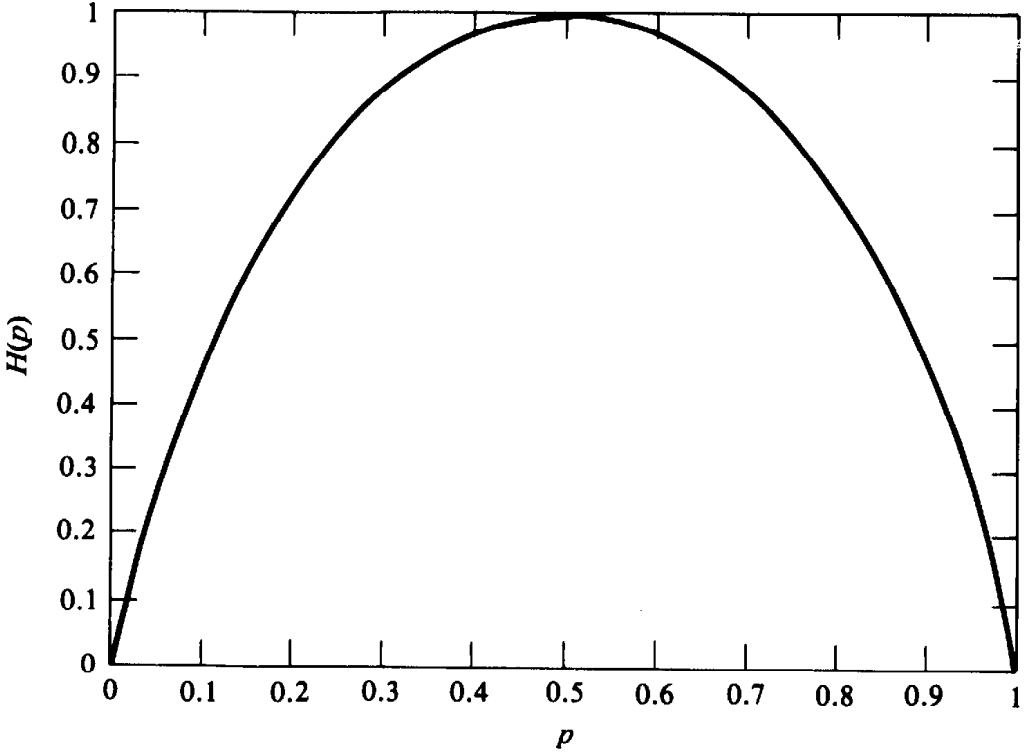
\includegraphics[width=0.5\linewidth]{Figures/H(p) versus p..png}
        \caption{H(p) versus p.}
        \label{fig:H(p) versus p.}
    \end{figure}

    The function \(H(p)\) is concave and symmetric around \(p = 0.5\), reaching its maximum of 1 bit/symbol at this point. When \(p = 0\) or \(p = 1\), there is no uncertainty, so \(H = 0\).
\end{questionanswerbox}

\begin{questionanswerbox}
\textbf{Q:} Why is probability multiplied with self-information in the entropy equation?

\medskip

\textbf{A:}

The probability of an event always lies in the range \(0 \le p(x) \le 1\).
However, the self-information
\[
I(x)=\log_2\!\left(\frac{1}{p(x)}\right)
\]
can be greater than 1 for low-probability events.

\medskip

\textbf{Examples:}
\begin{itemize}
    \item For \(p=0.8\): \(\log_2\!\left(\frac{1}{0.8}\right)\approx 0.32\)
    \item For \(p=0.3\): \(\log_2\!\left(\frac{1}{0.3}\right)\approx 1.73 > 1\)
\end{itemize}

\medskip

\textbf{Therefore,} to maintain the entropy value under 1 (and to obtain an average value), the self-information is multiplied by its probability.

\[
H(X)=\sum_x p(x)\,I(x)
\]

\textbf{Conclusion:}  
Probability \(p(x)\) is multiplied with self-information to maintain the entropy value under 1 and to compute the average information of the source.
\end{questionanswerbox}

\begin{questionanswerbox}
\textbf{Q:} If there are \(100\) equiprobable outcomes, calculate the corresponding
values of entropy in \textbf{bits}, \textbf{nats}, and \textbf{hartley}.

\medskip
\textbf{Given:} \(N = 100\) equiprobable outcomes.

\medskip
\textbf{A:}

\begin{itemize}
    \item \textbf{In bits:}
    \[
        H(X) = \log_2 100 \approx 6.64~\text{bits}
    \]

    \item \textbf{In nats:}
    \[
        H(X) = \log_e 100 = \ln 100 \approx 4.605~\text{nats}
    \]

    \item \textbf{In hartley:}
    \[
        H(X) = \log_{10} 100 = 2~\text{hartley}
    \]
\end{itemize}
\end{questionanswerbox}

\begin{questionanswerbox}
    \textbf{Example 2: Four-Symbol Source}

    Let \(X = \begin{cases}
        a & \text{with probability } 1/2 \\
        b & \text{with probability } 1/4 \\
        c & \text{with probability } 1/8 \\
        d & \text{with probability } 1/8
    \end{cases}\)

    The entropy is:
    \begin{align*}
        H(X) & = -\sum_{x \in \mathcal{X}} p(x) \log_2 p(x)                                                                             \\
             & = -\frac{1}{2}\log \frac{1}{2} - \frac{1}{4}\log \frac{1}{4} - \frac{1}{8}\log \frac{1}{8} - \frac{1}{8}\log \frac{1}{8} \\
             & = -\frac{1}{2}(-1) - \frac{1}{4}(-2) - \frac{1}{8}(-3) - \frac{1}{8}(-3)                                                 \\
             & = \frac{1}{2} + \frac{1}{2} + \frac{3}{8} + \frac{3}{8}                                                                  \\
             & = \frac{7}{4} = 1.75 \text{ bits}
    \end{align*}

    \textbf{Note:} \\
    Here L = 4\\
    If all probabilities were equal (\(p = 1/L = 1/4\) for all), then:
    \[
        H(X) = -4 \cdot \frac{1}{4}\log_2 \frac{1}{4} = \log_2 4 = 2 \text{ bits}
    \]

    This shows that when probabilities are not uniform, entropy is less than maximum, and information and entropy is maximized with equal probabilities.
\end{questionanswerbox}

\begin{questionanswerbox}
\textbf{Q:}\\
A source generates information with probabilities
\[
P_1 = 0.1,\quad P_2 = 0.2,\quad P_3 = 0.3,\quad P_4 = 0.4.
\]
Find the entropy of the source. What ercentage of maximum possible information is being generated by the source?\\
\textbf{A:}\\

\textbf{(a) Entropy of the source}
The entropy of a discrete source is given by:
\[
H(X) = -\sum_{i=1}^{n} p_i \log_2 p_i
\]

Substituting the given probabilities:
\begin{align*}
H(X)
&= -\Big[
0.1\log_2(0.1)
+ 0.2\log_2(0.2)
+ 0.3\log_2(0.3)
+ 0.4\log_2(0.4)
\Big] \\
&= 1.8464 \ \text{bits/symbol}
\end{align*}

\textbf{(b) Percentage of maximum possible information generated}

For a source with \(n=4\) symbols, for maximum entropy all probabilities are equal, (\(p = 1/L = 1/4\) for all), then:
\[
H_{\max} = -4 \cdot \frac{1}{4}\log_2 \frac{1}{4} = \log_2 4 = 2 \text{ bits/symbol}
\]

The efficiency (percentage of maximum information) is:
\[
\eta = \frac{H}{H_{\max}} \times 100
\]

\[
\eta = \frac{1.8464}{2} \times 100 = 92.32\%
\]

\textbf{Final Answer:}
\begin{itemize}
    \item Entropy of the source: \(\boxed{H(X) = 1.8464 \ \text{bits/symbol}}\)
    \item Percentage of maximum possible information: \(\boxed{92.32\%}\)
\end{itemize}

\end{questionanswerbox}

\begin{questionanswerbox}
\textbf{Q:} Calculate the entropy of the QPSK transmitted signal given below:

\[
00\; 01\; 10\; 10\; 11\; 11\; 01\; 01\; 10\; 00\; 10\; 10\; 11\; 01\; 10
\]

\medskip
\textbf{A:}

QPSK has four distinct bit combinations:
\[
(00,\;01,\;10,\;11)
\]

Hence,
\[
2^n = 4 \Rightarrow n = 2
\]
So, each symbol consists of two bits.

\medskip
\textbf{Frequency of symbols:}

\renewcommand{\arraystretch}{1.4}
\setlength{\tabcolsep}{6pt}
\newcolumntype{C}[1]{>{\centering\arraybackslash}m{#1}}

\begin{longtable}{|C{4cm}|C{3cm}|}
\hline
\rowcolor{gray!25}
\textbf{Symbol} & \textbf{Times} \\
\hline
\endhead

00 & 2 \\
\hline
01 & 4 \\
\hline
10 & 6 \\
\hline
11 & 3 \\
\hline

\caption{Symbol Occurrence Count for QPSK Signal}
\label{tab:qpsk_symbol_times}
\end{longtable}


Total number of symbols \(= 15\).

\medskip
\textbf{Probabilities:}
\[
p_{00} = \frac{2}{15}, \quad
p_{01} = \frac{4}{15}, \quad
p_{10} = \frac{6}{15}, \quad
p_{11} = \frac{3}{15}
\]

\medskip
\textbf{Entropy calculation:}

\begin{align*}
H(X) &= -\Big[
p_{00}\log_2 p_{00}
+ p_{01}\log_2 p_{01}
+ p_{10}\log_2 p_{10}
+ p_{11}\log_2 p_{11}
\Big] \\
&= -\Big[
\frac{2}{15}\log_2\frac{2}{15}
+ \frac{4}{15}\log_2\frac{4}{15}
+ \frac{6}{15}\log_2\frac{6}{15}
+ \frac{3}{15}\log_2\frac{3}{15}
\Big] \\
&= 1.889 \approx 2~\text{bits/symbol}
\end{align*}

\medskip
\textbf{Physical significance:}  
Thus, at least \textbf{2 bits per symbol} are required to transmit the QPSK signal.
\end{questionanswerbox}

\begin{questionanswerbox}
\textbf{Q:} Calculate the entropy of the finite length discrete memoryless source \(X\) with
probability distribution
\[
p(x)=\{0.125,\;0.25,\;0.5,\;0.125\}, \quad x\in\mathcal{X}.
\]

\medskip\\
\textbf{A:}
\medskip\\

\textbf{Given:}
\[
p(x)=\{0.125,\;0.25,\;0.5,\;0.125\}
\]

The entropy of a discrete memoryless source is:
\[
H(X)= -\sum_{i=1}^{n} p_i \log_2 p_i
\]

Substituting the values:

\begin{align*}
H(X)
&= -\Big[0.125\log_2(0.125)
+0.25\log_2(0.25)
+0.5\log_2(0.5)
+0.125\log_2(0.125)\Big] \\[6pt]
&= -\Big[2(0.125\log_2 0.125)
+0.25\log_2 0.25
+0.5\log_2 0.5\Big] \\[6pt]
&= 1.375 \ \text{bits}.
\end{align*}

\textbf{Answer:}
\[
H(X)=1.375\ \text{bits}
\]
\end{questionanswerbox}

\begin{questionanswerbox}
\textbf{Q:} For a source \(X\) with probability mass function
\[
p(x)=\{0.0625,\;0.5,\;0.25,\;0.125,\;0.0625\},
\]
calculate the average self-information of the source.

\medskip\\
\textbf{A:}
\medskip\\

\textbf{Given:}
\[
p(x)=\{0.0625,\;0.5,\;0.25,\;0.125,\;0.0625\}
\]

The average self-information of a source is equal to its entropy:
\[
H(X)= -\sum_{i=1}^{n} p_i \log_2 p_i
\]

\begin{align*}
H(X)
&= -\Big[
2(0.0625\log_2 0.0625)
+0.5\log_2 0.5
+0.25\log_2 0.25
+0.125\log_2 0.125
\Big] \\[6pt]
&= 1.875 \ \text{bits}.
\end{align*}

\textbf{Answer:}
\[
\text{Average self-information} = 1.875\ \text{bits}
\]
\end{questionanswerbox}

\begin{questionanswerbox}
\textbf{Q:} An 8-PSK modulator generates the following bit sequence:
\[
010,\;110,\;111,\;101,\;011,\;000,\;011,\;101,\;110,\;101,\;110,\;111,\;010,\;001,\;101,\;100.
\]
Determine the average information of the modulator.

\medskip\\
\textbf{A:}
\medskip\\
\textbf{Given:}

An 8-PSK modulator has \(2^3 = 8\) possible symbols, each represented by 3 bits.
From the given sequence, the symbol occurrences are:

\renewcommand{\arraystretch}{1.4}
\setlength{\tabcolsep}{6pt}
\newcolumntype{C}[1]{>{\centering\arraybackslash}m{#1}}

\begin{longtable}{|C{4cm}|C{3cm}|}
\hline
\rowcolor{gray!25}
\textbf{Symbol} & \textbf{Count} \\
\hline
\endhead

000 & 1 \\
\hline
001 & 1 \\
\hline
010 & 2 \\
\hline
011 & 2 \\
\hline
100 & 1 \\
\hline
101 & 4 \\
\hline
110 & 3 \\
\hline
111 & 2 \\
\hline
\rowcolor{gray!15}
\textbf{Total} & \textbf{16} \\
\hline

\caption{Symbol Frequency Table for 8-PSK Modulated Sequence}
\label{tab:8psk_symbol_count}
\end{longtable}

Hence, the probabilities are:
\[
p = \left\{\frac{1}{16},\;\frac{1}{16},\;\frac{2}{16},\;\frac{2}{16},\;\frac{1}{16},\;\frac{4}{16},\;\frac{3}{16},\;\frac{2}{16}\right\}
\]

\medskip

\textbf{Average information (Entropy):}
\[
H = -\sum p_i \log_2 p_i
\]

\begin{align*}
H
&= -\Big[
3\!\left(\tfrac{1}{16}\log_2\tfrac{1}{16}\right)
+3\!\left(\tfrac{2}{16}\log_2\tfrac{2}{16}\right)
+\tfrac{3}{16}\log_2\tfrac{3}{16}
+\tfrac{4}{16}\log_2\tfrac{4}{16}
\Big] \\[6pt]
&\approx 2.8278\ \text{bits/symbol}.
\end{align*}

\medskip

\textbf{Answer:}
\[
\boxed{\text{Average information} \approx 2.83\ \text{bits/symbol} \approx 3\ \text{bits/symbol}}
\]

\medskip

\textbf{Significance:}

At least \(\boxed{3}\) bits are required to transmit the 8-PSK modulated signal.
\end{questionanswerbox}

\begin{formulabox}[Average information rate]
    \[
R = H(X)\times r
\]
\textbf{Here:}
\begin{itemize}
    \item \(R\) = Average information rate = Total number of information bits produced by the source per second (bits/sec).
    \item \(H(X)\) = Entropy of the source = Average number of bits required to represent one symbol generated by the source (bits/symbol).
    \item \(r\) = Symbol emission rate = Number of symbols produced by the source per second (symbols/sec).
\end{itemize}

\end{formulabox}

\begin{questionanswerbox}
\textbf{Q:}
The output of an information source consists of \(150\) symbols, \(32\) of which
occur with a probability of \(\frac{1}{64}\) and the remaining with a probability
of \(\frac{1}{236}\).  
The source emits \(2000\) symbols per second.  
Assuming the symbols are chosen independently, find the average information
rate of this source.

\medskip\\
\textbf{A:}
\medskip\\
\textbf{Given:}
\[
p_1=\frac{1}{64}, \quad p_2=\frac{1}{236},
\qquad
n_1=32, \quad n_2=150-32=118
\]

\medskip

\textbf{Step 1: Entropy of the source}

The entropy of the source is
\[
H(X)
= -\Big[
n_1\,p_1\log_2 p_1 + n_2\,p_2\log_2 p_2
\Big]
\]

Substituting the values:
\begin{align*}
H(X)
&= -\Big[
32\left(\frac{1}{64}\log_2\frac{1}{64}\right)
+118\left(\frac{1}{236}\log_2\frac{1}{236}\right)
\Big] \\[6pt]
&= -\big[-3 - 3.9413\big] \\[6pt]
&= 6.9413 \ \text{bits/symbol}.
\end{align*}

\medskip

\textbf{Step 2: Average information rate}

The average information rate is
\[
R = H(X)\times r
\]
where \(r=2000\) symbols/sec.

\begin{align*}
R
&= 6.9413 \times 2000 \\[6pt]
&= 13882.64305 \ \text{bits/sec}.
\end{align*}

\medskip

\textbf{Answer:}
\[
\boxed{R \approx 1.388\times 10^{4}\ \text{bits/sec}}
\]
\end{questionanswerbox}

\begin{questionanswerbox}
\textbf{Q:} A black-and-white TV picture consists of 525 lines of picture information.
Assume that each picture element can have 256 brightness levels.
Pictures are replaced at a rate of 32 frames per second.
Calculate the average rate of information conveyed by the TV set to a viewer.

\medskip\\
\textbf{A:}
\medskip\\
\textbf{Given:}
\begin{itemize}
    \item Frame rate \(= 32\) frames/sec
    \item Number of lines per frame \(= 525\)
    \item Number of pixels per line \(= 256\)
    \item Brightness levels per pixel \(= 256\)
    
\end{itemize}

\medskip

\textbf{Step 1: Pixels per frame}
\[
\text{Pixels per frame}
= 525 \times 256
= 134{,}400 \ \text{pixels/frame}
\]

\medskip

\textbf{Step 2: Bits per pixel}

Since each pixel has 256 brightness levels,
\[
\text{Bits per pixel} = \log_2 256 = 8 \ \text{bits}
\]

\medskip

\textbf{Step 3: Bits per frame}
\[
\text{Bits per frame}
= 134{,}400 \times 8
= 1{,}075{,}200 \ \text{bits/frame}
\]

\medskip

\textbf{Step 4: Information rate}
\[
R = (\text{bits per frame}) \times (\text{frames per second})
\]
\[
R = 1{,}075{,}200 \times 32
= 34{,}406{,}400 \ \text{bits/sec}
\]

\medskip

\textbf{Answer:}
\[
\boxed{R \approx 34.4 \ \text{Mbps}}
\]
\end{questionanswerbox}

\subsection{Joint Entropy}

\begin{definitionbox}[Joint Entropy]
    The joint entropy \(H(X,Y)\) of a pair of discrete random variables \((X,Y)\) with joint distribution \(p(x,y)\) is defined as:
    \[
        H(X,Y) = -\sum_{x \in \mathcal{X}} \sum_{y \in \mathcal{Y}} p(x,y) \log p(x,y)
    \]

    Alternatively:
    \[
        H(X,Y) = -E \log p(X,Y)
    \]
\end{definitionbox}

\subsubsection{Properties of Joint Entropy}
\begin{infobox}[Properties of Joint Entropy]
    \begin{itemize}
        \item \(H(X,Y) \geq 0\)
        \item \(H(X,Y) = H(X) + H(Y)\) if and only if \(X\) and \(Y\) are independent
        \item \(H(X,Y) < H(X) + H(Y)\) (inequality for dependence)
    \end{itemize}
\end{infobox}

\begin{questionanswerbox}
\textbf{Q:} Two variables \(X\) (study hours) and \(Y\) (attendance) for a student have
their joint probabilities listed below. Show that the variables are dependent.

\medskip
\textbf{Given:}

\begin{center}
\begin{tabular}{|c|c|c|}
\hline
\textbf{X (Study Hours)} & \textbf{Y (Attendance)} & \(\mathbf{P(X,Y)}\) \\
\hline
Low  & Low  & 0.20 \\
Low  & High & 0.10 \\
High & Low  & 0.15 \\
High & High & 0.55 \\
\hline
\end{tabular}
\end{center}

\medskip
\textbf{A:}\\
\textbf{Joint entropy for each case:}

\begin{align*}
H_{LL}(X,Y) &= -0.20 \log_2 0.20 = 0.46 \\
H_{LH}(X,Y) &= -0.10 \log_2 0.10 = 0.33 \\
H_{HL}(X,Y) &= -0.15 \log_2 0.15 = 0.41 \\
H_{HH}(X,Y) &= -0.55 \log_2 0.55 = 0.4743
\end{align*}

\medskip
\textbf{Total joint entropy:}
\[
H(X,Y) = 0.46 + 0.33 + 0.41 + 0.4743 = 1.6743
\]

%--------------------------------------------------
\medskip
\textbf{Marginal entropy of study hours \(X\):}

\[
P_L = 0.20 + 0.10 = 0.30,
\qquad
P_H = 0.15 + 0.55 = 0.70
\]

\begin{align*}
H(X)
&= -\big[ P_L \log_2 P_L + P_H \log_2 P_H \big] \\
&= -\big[ 0.30 \log_2 0.30 + 0.70 \log_2 0.70 \big] \\
&= 0.881
\end{align*}

%--------------------------------------------------
\medskip
\textbf{Marginal entropy of attendance \(Y\):}

\[
P_L = 0.20 + 0.15 = 0.35,
\qquad
P_H = 0.10 + 0.55 = 0.65
\]

\begin{align*}
H(Y)
&= -\big[ P_L \log_2 P_L + P_H \log_2 P_H \big] \\
&= -\big[ 0.35 \log_2 0.35 + 0.65 \log_2 0.65 \big] \\
&= 0.934
\end{align*}

%--------------------------------------------------
\medskip
\textbf{Comparison:}
\[
H(X) + H(Y) = 0.881 + 0.934 = 1.815
\]

Since
\[
H(X) + H(Y) > H(X,Y),
\]
the variables \(X\) and \(Y\) are \textbf{dependent}.

\medskip
\textbf{Conclusion:}  
The variables \(X\) and \(Y\) are dependent and therefore contain
\textbf{mutual information}.
\end{questionanswerbox}

\subsection{Conditional Entropy}

\begin{definitionbox}[Conditional Entropy]
    The conditional entropy \(H(Y|X)\) measures the average uncertainty remaining in \(Y\) when \(X\) is known:
    \[
        H(Y|X) = \sum_{x \in \mathcal{X}} p(x) \sum_{y \in \mathcal{Y}} p(y|x) \log p(y|x)
    \]

    Equivalently:
    \[
        H(Y|X) = -E \log p(Y|X)
    \]
\end{definitionbox}

\begin{formulabox}[Chain Rule for Conditional Entropy]

The chain rule for conditional entropy is given by:

\[
H(X_1, X_2, \ldots, X_n \mid Y)
= \sum_{i=1}^{n} H\!\left(X_i \mid X_1, X_2, \ldots, X_{i-1}, Y\right)
\]

\end{formulabox}

\subsection{Chain Rule for Entropy}
\begin{formulabox}[Chain Rule for Entropy]
\begin{itemize}[label=$\rightarrow$]
    \item \[
        H(X,Y) = H(X) + H(Y|X)
    \]

    \textbf{Interpretation:} Joint Entropy = Marginal Entropy + Conditional Entropy

    \item The entropy of a sequence of random variables
\(X_1, X_2, \ldots, X_n\) is given by the chain rule:

\[
H(X_1, X_2, \ldots, X_n)
= \sum_{i=1}^{n} H\!\left(X_i \mid X_1, X_2, \ldots, X_{i-1}\right)
\]

\textbf{Examples:}

\begin{itemize}
    \item For \(n = 2\):
    \[
        H(X_1, X_2) = H(X_1) + H(X_2 \mid X_1)
    \]

    \item For \(n = 3\):
    \[
        H(X_1, X_2, X_3)
        = H(X_1) + H(X_2 \mid X_1) + H(X_3 \mid X_1, X_2)
    \]
\end{itemize}
\end{itemize}
\end{formulabox}

\begin{derivationbox}[Proof of Chain Rule]
    Starting from the definition of joint entropy:
    \begin{align*}
        H(X,Y) & = -\sum_{x \in \mathcal{X}} \sum_{y \in \mathcal{Y}} p(x,y) \log p(x,y) \\
               & = -\sum_{x,y} p(x,y) \log [p(x)p(y|x)]                                  \\
               & = -\sum_{x,y} p(x,y) \log p(x) - \sum_{x,y} p(x,y) \log p(y|x)          \\
               & = -\sum_{x} p(x) \log p(x) - \sum_{x,y} p(x,y) \log p(y|x)              \\
               & = H(X) + H(Y|X)
    \end{align*}
\end{derivationbox}

\begin{questionanswerbox}
[Complex method; Read it if you want to learn,otherwise look Example \ref{Finding_Find H(X), H(Y), H(X,Y), H(X|Y), H(Y|X)}]\\
    \textbf{Q:} Let \((X,Y)\) have the following joint distribution:

    \begin{center}
        \begin{tabular}{c|cccc|c}
            \(Y \backslash X\) & 1    & 2    & 3    & 4    & \(p(Y)\) \\ \hline
            1                  & 1/8  & 1/16 & 1/32 & 1/32 & 1/4      \\
            2                  & 1/16 & 1/8  & 1/32 & 1/32 & 1/4      \\
            3                  & 1/16 & 1/16 & 1/16 & 1/16 & 1/4      \\
            4                  & 1/4  & 0    & 0    & 0    & 1/4      \\ \hline
            \(p(X)\)           & 1/2  & 1/4  & 1/8  & 1/8  & 1
        \end{tabular}
    \end{center}

    Find H(X), H(Y), H(X,Y), H(X|Y), H(Y|X).
    \\ \\
    \textbf{A:}

    \textbf{Step 1: Calculate Marginal Entropy \(H(X)\)}

    Marginal distribution of \(X\): \(p(X) = \left(\frac{1}{2}, \frac{1}{4}, \frac{1}{8}, \frac{1}{8}\right)\)

    \begin{align*}
        H(X) & = -\sum_{x} p(x) \log_2 p(x)                                                                                                     \\
             & = -\frac{1}{2}\log_2 \frac{1}{2} - \frac{1}{4}\log_2 \frac{1}{4} - \frac{1}{8}\log_2 \frac{1}{8} - \frac{1}{8}\log_2 \frac{1}{8} \\
             & = -\frac{1}{2}(-1) - \frac{1}{4}(-2) - \frac{1}{8}(-3) - \frac{1}{8}(-3)                                                         \\
             & = \frac{1}{2} + \frac{2}{4} + \frac{3}{8} + \frac{3}{8}                                                                          \\
             & = \frac{4}{8} + \frac{4}{8} + \frac{3}{8} + \frac{3}{8} = \frac{14}{8} = \frac{7}{4} \text{ bits}
    \end{align*}

    \textbf{Step 2: Calculate Marginal Entropy \(H(Y)\)}

    Marginal distribution of \(Y\): \(p(Y) = \left(\frac{1}{4}, \frac{1}{4}, \frac{1}{4}, \frac{1}{4}\right)\)

    \begin{align*}
        H(Y) & = -\sum_{y} p(y) \log_2 p(y)              \\
             & = -4 \times \frac{1}{4}\log_2 \frac{1}{4} \\
             & = -4 \times \frac{1}{4} \times (-2)       \\
             & = 2 \text{ bits}
    \end{align*}

    \textbf{Step 3: Calculate Conditional Entropy \(H(X|Y)\) and Joint Entropy \(H(X,Y)\)}

    The conditional entropy formula is:
    \[
        H(X|Y) = \sum_{i=1}^{4} p(Y=i) \cdot H(X|Y=i)
    \]

    This means: "Average the entropy of X for each fixed value of Y, weighted by probability of that Y."

    \begin{formulabox}[Bayes' rule]
        To find \(H(X|Y=i)\), we need the conditional probabilities \(p(X=j|Y=i)\).

        Using Bayes' rule: \(p(X=j|Y=i) = \frac{p(X=j, Y=i)}{p(Y=i)}\)
    \end{formulabox}

    \hrulefill

    \textbf{When \(Y=1\):} \(p(Y=1) = \frac{1}{4}\)

    Conditional probabilities from the joint table:
    \begin{align*}
        p(X=1|Y=1) & = \frac{p(X=1,Y=1)}{p(Y=1)} = \frac{1/8}{1/4} = \frac{1}{2}  \\
        p(X=2|Y=1) & = \frac{p(X=2,Y=1)}{p(Y=1)} = \frac{1/16}{1/4} = \frac{1}{4} \\
        p(X=3|Y=1) & = \frac{p(X=3,Y=1)}{p(Y=1)} = \frac{1/32}{1/4} = \frac{1}{8} \\
        p(X=4|Y=1) & = \frac{p(X=4,Y=1)}{p(Y=1)} = \frac{1/32}{1/4} = \frac{1}{8}
    \end{align*}

    \textbf{Verification:} \(\frac{1}{2} + \frac{1}{4} + \frac{1}{8} + \frac{1}{8} = 1\) ✓

    Now calculate entropy:
    \begin{align*}
        H(X|Y=1) & = -\sum_{j=1}^{4} p(X=j|Y=1) \log_2 p(X=j|Y=1)                                                                               \\
                 & = -\frac{1}{2}\log_2\frac{1}{2} - \frac{1}{4}\log_2\frac{1}{4} - \frac{1}{8}\log_2\frac{1}{8} - \frac{1}{8}\log_2\frac{1}{8} \\
                 & = -\frac{1}{2}(-1) - \frac{1}{4}(-2) - \frac{1}{8}(-3) - \frac{1}{8}(-3)                                                     \\
                 & = \frac{1}{2} + \frac{1}{2} + \frac{3}{8} + \frac{3}{8} = \frac{7}{4} \text{ bits}
    \end{align*}

    \hrulefill

    \textbf{When \(Y=2\):} \(p(Y=2) = \frac{1}{4}\)

    Conditional probabilities:
    \begin{align*}
        p(X=1|Y=2) & = \frac{1/16}{1/4} = \frac{1}{4}, \quad
        p(X=2|Y=2) = \frac{1/8}{1/4} = \frac{1}{2}           \\
        p(X=3|Y=2) & = \frac{1/32}{1/4} = \frac{1}{8}, \quad
        p(X=4|Y=2) = \frac{1/32}{1/4} = \frac{1}{8}
    \end{align*}

    Entropy:
    \begin{align*}
        H(X|Y=2) & = -\frac{1}{4}\log_2\frac{1}{4} - \frac{1}{2}\log_2\frac{1}{2} - \frac{1}{8}\log_2\frac{1}{8} - \frac{1}{8}\log_2\frac{1}{8} \\
                 & = \frac{1}{2} + \frac{1}{2} + \frac{3}{8} + \frac{3}{8} = \frac{7}{4} \text{ bits}
    \end{align*}

    \hrulefill

    \textbf{When \(Y=3\):} \(p(Y=3) = \frac{1}{4}\)

    Conditional probabilities:
    \begin{align*}
        p(X=1|Y=3) & = \frac{1/16}{1/4} = \frac{1}{4}, \quad
        p(X=2|Y=3) = \frac{1/16}{1/4} = \frac{1}{4}          \\
        p(X=3|Y=3) & = \frac{1/16}{1/4} = \frac{1}{4}, \quad
        p(X=4|Y=3) = \frac{1/16}{1/4} = \frac{1}{4}
    \end{align*}

    Entropy (uniform distribution):
    \begin{align*}
        H(X|Y=3) & = -4 \times \frac{1}{4}\log_2\frac{1}{4} = -4 \times \frac{1}{4} \times (-2) = 2 \text{ bits}
    \end{align*}

    \hrulefill

    \textbf{When \(Y=4\):} \(p(Y=4) = \frac{1}{4}\)

    Conditional probabilities:
    \begin{align*}
        p(X=1|Y=4) & = \frac{1/4}{1/4} = 1, \quad
        p(X=2|Y=4) = \frac{0}{1/4} = 0            \\
        p(X=3|Y=4) & = \frac{0}{1/4} = 0, \quad
        p(X=4|Y=4) = \frac{0}{1/4} = 0
    \end{align*}

    Entropy (deterministic - no uncertainty):
    \begin{align*}
        H(X|Y=4) & = -1 \cdot \log_2 1 - 0 \cdot \log_2 0 - 0 \cdot \log_2 0 - 0 \cdot \log_2 0 \\
                 & = 0 \text{ bits (X is always 1 when Y=4)}
    \end{align*}

    \hrulefill

    \textbf{Now combine all cases:}
    \begin{align*}
        H(X|Y) & = \sum_{i=1}^{4} p(Y=i) \cdot H(X|Y=i)                                                                          \\
               & = p(Y=1) \cdot H(X|Y=1) + p(Y=2) \cdot H(X|Y=2)                                                                 \\
               & \quad + p(Y=3) \cdot H(X|Y=3) + p(Y=4) \cdot H(X|Y=4)                                                           \\
               & = \frac{1}{4} \times \frac{7}{4} + \frac{1}{4} \times \frac{7}{4} + \frac{1}{4} \times 2 + \frac{1}{4} \times 0 \\
               & = \frac{7}{16} + \frac{7}{16} + \frac{8}{16} + 0                                                                \\
               & = \frac{22}{16} = \frac{11}{8} \text{ bits}
    \end{align*}

    \textbf{Finally, using the chain rule:}
    \[
        H(X,Y) = H(Y) + H(X|Y) = 2 + \frac{11}{8} = \frac{16}{8} + \frac{11}{8} = \frac{27}{8} \text{ bits}
    \]

    \textbf{Step 4: Calculate \(H(Y|X)\)}

    Similarly, using: \(H(X,Y) = H(X) + H(Y|X)\)
    \[
        H(Y|X) = H(X,Y) - H(X) = \frac{27}{8} - \frac{7}{4} = \frac{27}{8} - \frac{14}{8} = \frac{13}{8} \text{ bits}
    \]

    \textbf{Summary of Results:}
    \begin{itemize}
        \item \(H(X) = \frac{7}{4} = 1.75\) bits
        \item \(H(Y) = 2\) bits
        \item \(H(X,Y) = \frac{27}{8} = 3.375\) bits
        \item \(H(X|Y) = \frac{11}{8} = 1.375\) bits
        \item \(H(Y|X) = \frac{13}{8} = 1.625\) bits
    \end{itemize}

    \textbf{Verification:}
    \begin{itemize}
        \item \(H(X,Y) = H(X) + H(Y|X) = \frac{7}{4} + \frac{13}{8} = \frac{14}{8} + \frac{13}{8} = \frac{27}{8}\) ✓
        \item \(H(X,Y) = H(Y) + H(X|Y) = 2 + \frac{11}{8} = \frac{16}{8} + \frac{11}{8} = \frac{27}{8}\) ✓
    \end{itemize}
\end{questionanswerbox}

\begin{questionanswerbox}
\label{Finding_Find H(X), H(Y), H(X,Y), H(X|Y), H(Y|X)}
    [Easier calculation than previous one]\\
    \textbf{Q:} Let \((X,Y)\) have the following joint distribution:

    \begin{center}
        \begin{tabular}{c|cccc|c}
            \(Y \backslash X\) & 1    & 2    & 3    & 4    & \(p(Y)\) \\ \hline
            1                  & 1/8  & 1/16 & 1/32 & 1/32 & 1/4      \\
            2                  & 1/16 & 1/8  & 1/32 & 1/32 & 1/4      \\
            3                  & 1/16 & 1/16 & 1/16 & 1/16 & 1/4      \\
            4                  & 1/4  & 0    & 0    & 0    & 1/4      \\ \hline
            \(p(X)\)           & 1/2  & 1/4  & 1/8  & 1/8  & 1
        \end{tabular}
    \end{center}

    Find H(X), H(Y), H(X,Y), H(X|Y), H(Y|X).
    \\
    \begin{formulabox}[Key Formulas]
        \begin{itemize}
            \item Marginal Entropy: \(H(X) = -\sum_{x} p(x) \log_2 p(x)\)
            \item Joint Entropy: \(H(X,Y) = -\sum_{x,y} p(x,y) \log_2 p(x,y)\)
            \item Chain Rule: \(H(X,Y) = H(X) + H(Y|X) = H(Y) + H(X|Y)\)
            \item Conditional Entropy: \(H(X|Y) = H(X,Y) - H(Y)\) and \(H(Y|X) = H(X,Y) - H(X)\)
            
        \end{itemize}
    \end{formulabox}
    \vspace{10pt}
    \textbf{Step 1: Calculate Marginal Entropy \(H(X)\)}

    Marginal distribution of \(X\): \(p(X) = \left(\frac{1}{2}, \frac{1}{4}, \frac{1}{8}, \frac{1}{8}\right)\)

    \begin{align*}
        H(X) & = -\sum_{x} p(x) \log_2 p(x)                                                                                                     \\
             & = -\frac{1}{2}\log_2 \frac{1}{2} - \frac{1}{4}\log_2 \frac{1}{4} - \frac{1}{8}\log_2 \frac{1}{8} - \frac{1}{8}\log_2 \frac{1}{8} \\
             & = -\frac{1}{2}(-1) - \frac{1}{4}(-2) - \frac{1}{8}(-3) - \frac{1}{8}(-3)                                                         \\
             & = \frac{1}{2} + \frac{2}{4} + \frac{3}{8} + \frac{3}{8}                                                                          \\
             & = \frac{4}{8} + \frac{4}{8} + \frac{3}{8} + \frac{3}{8} = \frac{14}{8} = \frac{7}{4} \text{ bits}
    \end{align*}
    \\
    \textbf{Step 2: Calculate Marginal Entropy \(H(Y)\)}

    Marginal distribution of \(Y\): \(p(Y) = \left(\frac{1}{4}, \frac{1}{4}, \frac{1}{4}, \frac{1}{4}\right)\)

    \begin{align*}
        H(Y) & = -\sum_{y} p(y) \log_2 p(y)              \\
             & = -4 \times \frac{1}{4}\log_2 \frac{1}{4} \\
             & = -4 \times \frac{1}{4} \times (-2)       \\
             & = 2 \text{ bits}
    \end{align*}
    \\
    \textbf{Step 3: Calculate Joint Entropy \(H(X,Y)\) Directly}

    Using the formula: \(H(X,Y) = -\sum_{x,y} p(x,y) \log_2 p(x,y)\)

    We sum over all non-zero entries in the joint distribution table:

    \begin{align*}
        H(X,Y) & = -\sum_{x,y} p(x,y) \log_2 p(x,y)                                                                                                        \\
               & = -\frac{1}{8}\log_2\frac{1}{8} - \frac{1}{16}\log_2\frac{1}{16} - \frac{1}{32}\log_2\frac{1}{32} - \frac{1}{32}\log_2\frac{1}{32}        \\
               & \quad - \frac{1}{16}\log_2\frac{1}{16} - \frac{1}{8}\log_2\frac{1}{8} - \frac{1}{32}\log_2\frac{1}{32} - \frac{1}{32}\log_2\frac{1}{32}   \\
               & \quad - \frac{1}{16}\log_2\frac{1}{16} - \frac{1}{16}\log_2\frac{1}{16} - \frac{1}{16}\log_2\frac{1}{16} - \frac{1}{16}\log_2\frac{1}{16} \\
               & \quad - \frac{1}{4}\log_2\frac{1}{4}
    \end{align*}

    Group by probability values:
    \begin{align*}
        H(X,Y) & = -\left[2 \times \frac{1}{8}\log_2\frac{1}{8} + 6 \times \frac{1}{16}\log_2\frac{1}{16} + 4 \times \frac{1}{32}\log_2\frac{1}{32} + 1 \times \frac{1}{4}\log_2\frac{1}{4}\right] \\
               & = -\left[2 \times \frac{1}{8} \times (-3) + 6 \times \frac{1}{16} \times (-4) + 4 \times \frac{1}{32} \times (-5) + 1 \times \frac{1}{4} \times (-2)\right]                       \\
               & = -\left[-\frac{6}{8} - \frac{24}{16} - \frac{20}{32} - \frac{2}{4}\right]                                                                                                        \\
               & = \frac{6}{8} + \frac{24}{16} + \frac{20}{32} + \frac{2}{4}                                                                                                                       \\
               & = \frac{108}{32} = \frac{27}{8} \text{ bits}
    \end{align*}
    \\
    \textbf{Step 4: Calculate \(H(X|Y)\) Using Formula}

    Using the chain rule: \(H(X|Y) = H(X,Y) - H(Y)\)

    \begin{align*}
        H(X|Y) & = H(X,Y) - H(Y)               \\
               & = \frac{27}{8} - 2            \\
               & = \frac{27}{8} - \frac{16}{8} \\
               & = \frac{11}{8} \text{ bits}
    \end{align*}
    \\
    \textbf{Step 5: Calculate \(H(Y|X)\) Using Formula}

    Using the chain rule: \(H(Y|X) = H(X,Y) - H(X)\)

    \begin{align*}
        H(Y|X) & = H(X,Y) - H(X)               \\
               & = \frac{27}{8} - \frac{7}{4}  \\
               & = \frac{27}{8} - \frac{14}{8} \\
               & = \frac{13}{8} \text{ bits}
    \end{align*}

    \textbf{Summary of Results:}
    \begin{itemize}
        \item \(H(X) = \frac{7}{4} = 1.75\) bits
        \item \(H(Y) = 2\) bits
        \item \(H(X,Y) = \frac{27}{8} = 3.375\) bits
        \item \(H(X|Y) = \frac{11}{8} = 1.375\) bits
        \item \(H(Y|X) = \frac{13}{8} = 1.625\) bits
    \end{itemize}

    \textbf{Verification:}
    \begin{itemize}
        \item \(H(X,Y) = H(X) + H(Y|X) = \frac{7}{4} + \frac{13}{8} = \frac{14}{8} + \frac{13}{8} = \frac{27}{8}\) ✓
        \item \(H(X,Y) = H(Y) + H(X|Y) = 2 + \frac{11}{8} = \frac{16}{8} + \frac{11}{8} = \frac{27}{8}\) ✓
    \end{itemize}
\end{questionanswerbox}

\begin{infobox}[Important Observations]
    \begin{itemize}
        \item \(H(Y|X) \neq H(X|Y)\) — Conditional entropies are generally not equal
        \item However, \(H(X) - H(X|Y) = H(Y) - H(Y|X)\) — This symmetric property is mutual information \(I(X;Y)\), explored in the next section
        \item \(H(X|Y) < H(X)\) — Knowing \(Y\) reduces uncertainty about \(X\)
        \item \(H(Y|X) < H(Y)\) — Knowing \(X\) reduces uncertainty about \(Y\)
    \end{itemize}
\end{infobox}

\section{Relative Entropy}

\begin{definitionbox}[Relative Entropy (Kullback--Leibler Divergence)]
\begin{itemize}
    \item Entropy \(H(X)\) measures the uncertainty of a single random variable.
    \item Relative entropy (also called \textbf{Kullback--Leibler divergence}) extends this concept
          to measure the \textbf{difference} between two probability distributions.
    \item It is also known as a \textbf{loss function}, since it measures the loss incurred
          when an estimated distribution is used instead of the true distribution.
\end{itemize}

\begin{formulabox}[Relative Entropy / KL Divergence]
The \textbf{relative entropy} or \textbf{Kullback--Leibler (KL) divergence}
between two probability mass functions \(p(x)\) and \(q(x)\) is defined as:
\[
    D(p \| q) = \sum_{x \in \mathcal{X}} p(x)\log\frac{p(x)}{q(x)}
\]

where:
\begin{itemize}
    \item \(p(x)\) represents the \textbf{true probability distribution},
    \item \(q(x)\) represents the \textbf{estimated (or assumed) probability distribution}.
\end{itemize}

Equivalently, in expectation form:
\[
    D(p \| q) = E_p\!\left[\log\frac{p(X)}{q(X)}\right]
\]
\end{formulabox}

\textbf{Important properties:}
\begin{itemize}
    \item If \(p(x) = q(x)\) for all \(x\), then
          \[
              D(p \| q) = 0
          \]
    \item In particular,
          \[
              D(p \| p) = 0
          \]
          which means there is no loss when the estimated distribution matches the true distribution.
    \item Relative entropy is always non-negative:
          \[
              D(p \| q) \ge 0
          \]
\end{itemize}

\textbf{Convention:}
\begin{itemize}
    \item \(0 \log \frac{0}{q} = 0\)
    \item \(p \log \frac{p}{0} = \infty\)
\end{itemize}
\end{definitionbox}

%==================================================

\begin{infobox}[Interpretation of Relative Entropy]
\begin{itemize}
    \item Relative entropy \(D(p\|q)\) measures how far an assumed (estimated) distribution
          \(q(x)\) deviates from the true distribution \(p(x)\).
    \item A larger value of \(D(p\|q)\) indicates a larger deviation from the true distribution.
    \item If the distributions match exactly, there is no loss:
          \[
              D(p\|p)=0
          \]
    \item Example comparison:
          \[
              D(p\|A)=0.25 < D(p\|B)=1.25
          \]
          Hence, distribution \(B\) deviates more from the true distribution than \(A\).
    \item From a coding perspective, using \(q\) instead of the true distribution \(p\)
          requires extra bits:
          \[
              \text{Average code length} = H(p) + D(p\|q)
          \]
          Thus, \(D(p\|q)\) represents the \textbf{extra bits (loss)} due to an incorrect model.
\end{itemize}
\end{infobox}

\subsection{Properties of Relative Entropy}
\begin{infobox}[Properties of Relative Entropy]
    \begin{enumerate}
    \item \textbf{Non-negativity:} \(D(p \| q) \geq 0\)
    \item \textbf{Zero condition:} \(D(p \| q) = 0\) if and only if \(p(x) = q(x)\) for all \(x\)
    \item \textbf{Asymmetry:} \(D(p \| q) \neq D(q \| p)\) in general
    \item \textbf{Not a metric:} Does not satisfy the triangle inequality and is not symmetric
\end{enumerate}
\end{infobox}

\begin{questionanswerbox}
    \textbf{Example 2.3.1: Binary Distributions with Different Parameters}

    Let \(\mathcal{X} = \{0, 1\}\) and consider two distributions \(p\) and \(q\) on \(\mathcal{X}\).

    \textbf{Given:}
    \begin{itemize}
        \item Distribution \(p\): \(p(0) = 1-r\), \(p(1) = r\)
        \item Distribution \(q\): \(q(0) = 1-s\), \(q(1) = s\)
    \end{itemize}

    \begin{formulabox}[General Formulas]

        The relative entropy from \(p\) to \(q\):
        \[
            D(p \| q) = (1-r) \log \frac{1-r}{1-s} + r \log \frac{r}{s}
        \]

        The relative entropy from \(q\) to \(p\):
        \[
            D(q \| p) = (1-s) \log \frac{1-s}{1-r} + s \log \frac{s}{r}
        \]
    \end{formulabox}

    \hrulefill

    \textbf{Special Case 1: Equal Distributions}

    If \(r = s\), then both distributions are identical:
    \[
        D(p \| q) = D(q \| p) = 0
    \]
    \textbf{Observation:} This confirms that relative entropy is zero when the distributions match.

    \hrulefill

    \textbf{Special Case 2: Specific Values}

    Let \(r = 1/2\) and \(s = 1/4\). Then:

    \textbf{Calculate \(D(p \| q)\):}
    \begin{align*}
        D(p \| q) & = (1-r) \log \frac{1-r}{1-s} + r \log \frac{r}{s}                     \\
                  & = \frac{1}{2} \log \frac{1/2}{3/4} + \frac{1}{2} \log \frac{1/2}{1/4} \\
                  & = \frac{1}{2} \log \frac{2}{3} + \frac{1}{2} \log 2                   \\
                  & = \frac{1}{2} \left(\log 2 - \log 3\right) + \frac{1}{2} \log 2       \\
                  & = \frac{1}{2} \log 2 - \frac{1}{2} \log 3 + \frac{1}{2} \log 2        \\
                  & = \log 2 - \frac{1}{2} \log 3                                         \\
                  & = 1 - \frac{1}{2} \log 3                                              \\
                  & \approx 1 - 0.7925 = 0.2075 \text{ bits}
    \end{align*}

    \textbf{Calculate \(D(q \| p)\):}
    \begin{align*}
        D(q \| p) & = (1-s) \log \frac{1-s}{1-r} + s \log \frac{s}{r}                     \\
                  & = \frac{3}{4} \log \frac{3/4}{1/2} + \frac{1}{4} \log \frac{1/4}{1/2} \\
                  & = \frac{3}{4} \log \frac{3}{2} + \frac{1}{4} \log \frac{1}{2}         \\
                  & = \frac{3}{4} (\log 3 - \log 2) + \frac{1}{4} (- \log 2)              \\
                  & = \frac{3}{4} \log 3 - \frac{3}{4} \log 2 - \frac{1}{4} \log 2        \\
                  & = \frac{3}{4} \log 3 - \log 2                                         \\
                  & = \frac{3}{4} \log 3 - 1                                              \\
                  & \approx 1.1887 - 1 = 0.1887 \text{ bits}
    \end{align*}

    \textbf{Observation:}
    \[
        D(p \| q) = 0.2075 \text{ bits} \neq D(q \| p) = 0.1887 \text{ bits}
    \]

    This demonstrates that \textbf{KL divergence is asymmetric} — the "distance" from \(p\) to \(q\) is different from the "distance" from \(q\) to \(p\).
\end{questionanswerbox}

\begin{questionanswerbox}
\textbf{Q:} Consider a scenario where the true distribution is:
\[
P_{\text{dog}} = 1, \qquad P_{\text{cat}} = 0
\]

Two estimated models are given:

\begin{itemize}
    \item \textbf{Model A:}
    \[
        P'_{\text{dog}} = 0.1, \qquad P'_{\text{cat}} = 0.9
    \]

    \item \textbf{Model B:}
    \[
        P''_{\text{dog}} = 0.9, \qquad P''_{\text{cat}} = 0.1
    \]
\end{itemize}

Find the relative entropy using the Kullback-Leibler divergence formula.\\

\textbf{A:}
\medskip\\
\textbf{KL divergence formula:}
\[
D(P\|Q) = \sum_x p(x)\log_2\!\left(\frac{p(x)}{q(x)}\right)
\]

%--------------------------------------------------
\textbf{For Model A:}

\[
D(P\|P') 
= P_{\text{dog}}\log_2\!\left(\frac{P_{\text{dog}}}{P'_{\text{dog}}}\right)
+ P_{\text{cat}}\log_2\!\left(\frac{P_{\text{cat}}}{P'_{\text{cat}}}\right)
\]

\[
= 1\log_2\!\left(\frac{1}{0.1}\right)
+ 0\log_2\!\left(\frac{0}{0.9}\right)
\]

\[
= \log_2 10
= 3.32 \text{ units}
\]

%--------------------------------------------------
\textbf{For Model B:}

\[
D(P\|P'') 
= P_{\text{dog}}\log_2\!\left(\frac{P_{\text{dog}}}{P''_{\text{dog}}}\right)
+ P_{\text{cat}}\log_2\!\left(\frac{P_{\text{cat}}}{P''_{\text{cat}}}\right)
\]

\[
= 1\log_2\!\left(\frac{1}{0.9}\right)
+ 0\log_2\!\left(\frac{0}{0.1}\right)
\]

\[
\approx 0.15 \text{ units}
\]

%--------------------------------------------------
\textbf{Conclusion:}

Since
\[
D(P\|P'') < D(P\|P'),
\]
\textbf{Model B is better} as it has lower KL divergence and is closer to the true distribution.
\end{questionanswerbox}

\begin{questionanswerbox}
\textbf{Q:}

Let \(\mathcal{X}=\{0,1\}\). Consider two distributions \(p\) and \(q\) on \(\mathcal{X}\) such that
\[
p(0)=1-\pi,\quad p(1)=\pi,
\qquad
q(0)=1-s,\quad q(1)=s.
\]
Find \(D(p\|q)\) and \(D(q\|p)\). Also verify that in general \(D(p\|q)\neq D(q\|p)\).
\medskip\\
\textbf{A:}
\medskip\\
\textbf{Given:}
\[
\mathcal{X}=\{0,1\},\quad
p(0)=1-\pi,\; p(1)=\pi,\quad
q(0)=1-s,\; q(1)=s.
\]

%--------------------------------------------------
\textbf{Step 1: Compute \(D(p\|q)\)}

\begin{align*}
D(p\|q)
&=\sum_{x\in\mathcal{X}} p(x)\log_2\left(\frac{p(x)}{q(x)}\right)\\[6pt]
&=p(0)\log_2\left(\frac{p(0)}{q(0)}\right)+p(1)\log_2\left(\frac{p(1)}{q(1)}\right)\\[6pt]
&=(1-\pi)\log_2\left(\frac{1-\pi}{1-s}\right)+\pi\log_2\left(\frac{\pi}{s}\right).
\end{align*}

%--------------------------------------------------
\textbf{Step 2: Compute \(D(q\|p)\)}

\begin{align*}
D(q\|p)
&=\sum_{x\in\mathcal{X}} q(x)\log_2\left(\frac{q(x)}{p(x)}\right)\\[6pt]
&=(1-s)\log_2\left(\frac{1-s}{1-\pi}\right)+s\log_2\left(\frac{s}{\pi}\right).
\end{align*}

\textbf{Step 3:} when \(\pi=s=\frac12\),
\[
D(p\|q)=0 \text{ and } D(q\|p)=0
\]

%--------------------------------------------------
\textbf{Step 4:} let \(\pi=\frac12\) and \(s=\frac14\)

\begin{align*}
D(p\|q)
&=\left(1-\frac12\right)\log_2\left(\frac{1-\frac12}{1-\frac14}\right)
+\left(\frac12\right)\log_2\left(\frac{\frac12}{\frac14}\right)\\[6pt]
&=\frac12\log_2\left(\frac{\frac12}{\frac34}\right)
+\frac12\log_2\left(\frac{\frac12}{\frac14}\right)\\[6pt]
&=\frac12\log_2\left(\frac{2}{3}\right)+\frac12\log_2(2)\\[6pt]
&=-0.292481+\frac12\\[6pt]
&=0.2075\ \text{bit}.
\end{align*}

\textbf{and}

\begin{align*}
D(q\|p)
&=\left(1-\frac14\right)\log_2\left(\frac{1-\frac14}{1-\frac12}\right)
+\left(\frac14\right)\log_2\left(\frac{\frac14}{\frac12}\right)\\[6pt]
&=\frac34\log_2\left(\frac{\frac34}{\frac12}\right)+\frac14\log_2\left(\frac12\right)\\[6pt]
&=\frac34\log_2\left(\frac{3}{2}\right)-\frac14\\[6pt]
&=0.438721-0.25\\[6pt]
&=0.188721\ \text{bit}.
\end{align*}

%--------------------------------------------------
\textbf{Conclusion:}
\[
D(p\|q)\neq D(q\|p)
\]
so the KL divergence is \textbf{not symmetric}.
\end{questionanswerbox}

\section{Mutual Information}

\begin{definitionbox}[Mutual Information]
\begin{itemize}
    \item Mutual information measures the amount of information one random variable X contains about another random variable Y.
    \item It quantifies the \textbf{reduction in uncertainty} of one variable due to knowledge of the other
\end{itemize}

\begin{formulabox}[Mutual Information]
    Consider two random variables \(X\) and \(Y\) with joint probability mass function \(p(x,y)\) and marginal probability mass functions \(p(x)\) and \(p(y)\).

    The \textbf{mutual information} \(I(X;Y)\) is the relative entropy between the joint distribution and the product distribution \(p(x)p(y)\):
    \[
        I(X;Y) = \sum_{x \in \mathcal{X}} \sum_{y \in \mathcal{Y}} p(x,y) \log \frac{p(x,y)}{p(x)p(y)}
    \]

    Equivalently:
    \[
        I(X;Y) = D(p(x,y) \| p(x)p(y))
    \]

    Or in expectation form:
    \[
        I(X;Y) = E_{p(x,y)} \log \frac{p(X,Y)}{p(X)p(Y)}
    \]
\end{formulabox}
    
\end{definitionbox}

\begin{infobox}[Interpretation of Mutual Information]
    \begin{itemize}
        \item \(I(X;Y)\) represents how much knowing \(Y\) reduces uncertainty about \(X\) (and vice versa)
        \item It measures the dependence between \(X\) and \(Y\)
        \item When \(X\) and \(Y\) are independent: \(I(X;Y) = 0\)
    \end{itemize}
\end{infobox}

\subsection{Relationship with Entropy}

\begin{formulabox}
    \[
        I(X;Y) = H(X) - H(X|Y)
    \]
    \begin{itemize}
        \item \(H(X)\) = Uncertainty about \(X\) before knowing \(Y\)
        \item \(H(X|Y)\) = Uncertainty about \(X\) after knowing \(Y\)
        \item \(I(X;Y)\) = Reduction in uncertainty = Information gained about \(X\) from \(Y\)
    \end{itemize}
\end{formulabox}

\begin{derivationbox}[Derivation: I(X;Y) = H(X) - H(X|Y)]
    We can rewrite the definition of mutual information \(I(X;Y)\) step by step:
\medskip\\
    \textbf{Step 1: Start from the definition}
\[
I(X;Y)=\sum_{x,y} p(x,y)\log\left(\frac{p(x,y)}{p(x)p(y)}\right)
\]

\textbf{Step 2: Use Baye's theorem \(p(x,y)=p(x)\,p(y|x)\)}
\[
\frac{p(x,y)}{p(x)p(y)}
=\frac{p(x)p(y|x)}{p(x)p(y)}
=\frac{p(y|x)}{p(y)}
\]

Hence,
\begin{align*}
I(X;Y)
&=\sum_{x,y} p(x,y)\log\left(\frac{p(y|x)}{p(y)}\right)\\[6pt]
&=\sum_{x,y} p(x,y)\log p(y|x)\;-\;\sum_{x,y} p(x,y)\log p(y)
\end{align*}

\textbf{Step 3: Convert each term into entropy}
\[
\sum_{x,y} p(x,y)\log p(y|x) = -H(Y|X)
\]
and since \(\log p(y)\) does not depend on \(x\),
\[
\sum_{x,y} p(x,y)\log p(y)=\sum_y p(y)\log p(y)=-H(Y)
\]

\textbf{Therefore,}
\[
\boxed{I(X;Y)=H(Y)-H(Y|X)}
\]

    \textbf{Step 4: Use joint entropy identity}
    \[
        H(X,Y)=H(X)+H(Y|X)
        \quad\Rightarrow\quad
        H(Y|X)=H(X,Y)-H(X)
    \]
    Substituting into \(I(X;Y)=H(Y)-H(Y|X)\),
    \[
        I(X;Y)=H(Y)-\big(H(X,Y)-H(X)\big)
        =\boxed{H(X)+H(Y)-H(X,Y)}
    \]
\end{derivationbox}

\begin{formulabox}[Mutual Information and Entropy]
The mutual information can be expressed in several equivalent forms:

\begin{align}
    I(X;Y) &= H(X) - H(X|Y) \label{eq:mi-x} \\[4pt]
    I(X;Y) &= H(Y) - H(Y|X) \label{eq:mi-y} \\[4pt]
    I(X;Y) &= H(X) + H(Y) - H(X,Y) \label{eq:mi-joint} \\[4pt]
    I(X;Y) &= I(Y;X) \quad \text{(symmetry)} \label{eq:mi-sym} \\[4pt]
    I(X;X) &= H(X) \label{eq:mi-self}
\end{align}

\textbf{Interpretations:}
\begin{itemize}
    \item \textbf{Equation \eqref{eq:mi-x}:} Mutual information = uncertainty in \(X\) minus uncertainty in \(X\) given \(Y\)
    \item \textbf{Equation \eqref{eq:mi-y}:} Mutual information = uncertainty in \(Y\) minus uncertainty in \(Y\) given \(X\)
    \item \textbf{Equation \eqref{eq:mi-joint}:} Mutual information = sum of marginal entropies minus joint entropy
    \item \textbf{Equation \eqref{eq:mi-sym}:} Mutual information is symmetric
    \item \textbf{Equation \eqref{eq:mi-self}:} A variable contains all information about itself
\end{itemize}
\end{formulabox}

\subsubsection{Venn Diagram Representation (Visual Understanding)}

The relationship between \(H(X)\), \(H(Y)\), \(H(X,Y)\), \(H(X|Y)\), \(H(Y|X)\), and \(I(X;Y)\) can be visualized as a Venn diagram (Figure 2.2):

\begin{figure}[H]
    \centering
    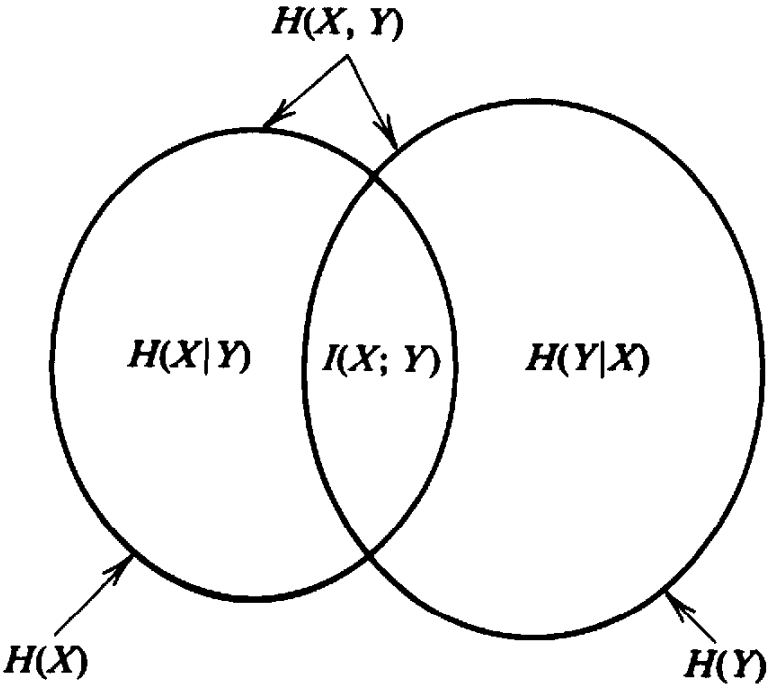
\includegraphics[width=0.3\linewidth]{Figures/Relationship between entropy and mutual information.png}
    \caption{Relationship between entropy and mutual information.}
    \label{fig:Relationship between entropy and mutual information.}
\end{figure}

\textbf{Key Observations:}
\begin{itemize}
    \item \textbf{Left circle}: Total uncertainty in \(X\) is \(H(X)\)
    \item \textbf{Right circle}: Total uncertainty in \(Y\) is \(H(Y)\)
    \item \textbf{Intersection}: Shared information is \(I(X;Y)\)
    \item \textbf{Left only}: Uncertainty in \(X\) after knowing \(Y\) is \(H(X|Y)\)
    \item \textbf{Right only}: Uncertainty in \(Y\) after knowing \(X\) is \(H(Y|X)\)
    \item \textbf{Total area}: Joint uncertainty is \(H(X,Y) = H(X|Y) + I(X;Y) + H(Y|X)\)
\end{itemize}

The mutual information corresponds to the intersection — the information that \(X\) and \(Y\) share.

\begin{formulabox}[Chain Rule for Mutual Information]

The chain rule for mutual information is:

\[
I(X_1, X_2, \ldots, X_n ; Y)
= \sum_{i=1}^{n} I\!\left(X_i ; Y \mid X_1, X_2, \ldots, X_{i-1}\right)
\]

\textbf{Examples:}

\begin{itemize}
    \item For \(n = 2\):
    \[
        I(X_1, X_2 ; Y)
        = I(X_1 ; Y) + I(X_2 ; Y \mid X_1)
    \]

    \item For \(n = 3\):
    \[
        I(X_1, X_2, X_3 ; Y)
        = I(X_1 ; Y)
        + I(X_2 ; Y \mid X_1)
        + I(X_3 ; Y \mid X_1, X_2)
    \]
\end{itemize}

\end{formulabox}

\begin{questionanswerbox}
    \textbf{Example: Mutual Information from Joint Distribution (Not in class note, made for understanding concept)}

    Using the joint distribution from Chapter 2:

    \begin{center}
        \begin{tabular}{c|cccc|c}
            \(Y \backslash X\) & 1    & 2    & 3    & 4    & \(p(Y)\) \\ \hline
            1                  & 1/8  & 1/16 & 1/32 & 1/32 & 1/4      \\
            2                  & 1/16 & 1/8  & 1/32 & 1/32 & 1/4      \\
            3                  & 1/16 & 1/16 & 1/16 & 1/16 & 1/4      \\
            4                  & 1/4  & 0    & 0    & 0    & 1/4      \\ \hline
            \(p(X)\)           & 1/2  & 1/4  & 1/8  & 1/8  & 1
        \end{tabular}
    \end{center}

    \textbf{Previously calculated values:}
    \begin{itemize}
        \item \(H(X) = \frac{7}{4} = 1.75\) bits
        \item \(H(Y) = 2\) bits
        \item \(H(X,Y) = \frac{27}{8} = 3.375\) bits
        \item \(H(X|Y) = \frac{11}{8} = 1.375\) bits
        \item \(H(Y|X) = \frac{13}{8} = 1.625\) bits
    \end{itemize}

    \hrulefill

    \textbf{Method 1: Using \(I(X;Y) = H(X) - H(X|Y)\)}
    \begin{align*}
        I(X;Y) & = H(X) - H(X|Y)                    \\
               & = \frac{7}{4} - \frac{11}{8}       \\
               & = \frac{14}{8} - \frac{11}{8}      \\
               & = \frac{3}{8} = 0.375 \text{ bits}
    \end{align*}

    \textbf{Method 2: Using \(I(X;Y) = H(Y) - H(Y|X)\)}
    \begin{align*}
        I(X;Y) & = H(Y) - H(Y|X)                    \\
               & = 2 - \frac{13}{8}                 \\
               & = \frac{16}{8} - \frac{13}{8}      \\
               & = \frac{3}{8} = 0.375 \text{ bits}
    \end{align*}

    \textbf{Method 3: Using \(I(X;Y) = H(X) + H(Y) - H(X,Y)\)}
    \begin{align*}
        I(X;Y) & = H(X) + H(Y) - H(X,Y)                       \\
               & = \frac{7}{4} + 2 - \frac{27}{8}             \\
               & = \frac{14}{8} + \frac{16}{8} - \frac{27}{8} \\
               & = \frac{30}{8} - \frac{27}{8}                \\
               & = \frac{3}{8} = 0.375 \text{ bits}
    \end{align*}

    \textbf{Interpretation:}
    \begin{itemize}
        \item Knowing \(Y\) reduces uncertainty about \(X\) by 0.375 bits
        \item Knowing \(X\) reduces uncertainty about \(Y\) by 0.375 bits
        \item The variables share 0.375 bits of information
        \item This is symmetric: \(I(X;Y) = I(Y;X)\) ✓
    \end{itemize}
\end{questionanswerbox}

\begin{questionanswerbox}
\textbf{Q:} Calculate the \textbf{joint entropy} for the following data and also find the
\textbf{mutual information}.

\medskip
\textbf{Given joint probability distribution:}

\begin{center}
\renewcommand{\arraystretch}{2.5}
\setlength{\tabcolsep}{10pt}

\begin{tabular}{|c|c|c|}
\hline
\rowcolor{gray!25}
\textbf{Y $\backslash$ X} & \textbf{0} & \textbf{1} \\
\hline
0 & $\dfrac{1}{2}$ & $\dfrac{1}{4}$ \\
\hline
1 & $\dfrac{1}{8}$ & $\dfrac{1}{8}$ \\
\hline
\end{tabular}
\end{center}


%--------------------------------------------------
\medskip
\textbf{Joint Entropy:}

\begin{align*}
H(X,Y) &= -\Big[
\frac{1}{2}\log_2\frac{1}{2}
+ \frac{1}{4}\log_2\frac{1}{4}
+ \frac{1}{8}\log_2\frac{1}{8}
+ \frac{1}{8}\log_2\frac{1}{8}
\Big] \\
&= \frac{1}{2}\log_2 2
+ \frac{1}{4}\log_2 4
+ \frac{1}{8}\log_2 8
+ \frac{1}{8}\log_2 8 \\
&= \frac{1}{2} + \frac{1}{2} + \frac{3}{4} \\
&= 1.75~\text{bits}
\end{align*}

%--------------------------------------------------
\medskip
\textbf{Marginal entropy of \(Y\):}

\[
P(Y=0)=\frac{1}{2}+\frac{1}{4}=\frac{3}{4},
\qquad
P(Y=1)=\frac{1}{8}+\frac{1}{8}=\frac{1}{4}
\]

\begin{align*}
H(Y)
&= -\Big[
\frac{3}{4}\log_2\frac{3}{4}
+ \frac{1}{4}\log_2\frac{1}{4}
\Big] \\
&= 0.811
\end{align*}

%--------------------------------------------------
\medskip
\textbf{Marginal entropy of \(X\):}

\[
P(X=0)=\frac{1}{2}+\frac{1}{8}=\frac{5}{8},
\qquad
P(X=1)=\frac{1}{4}+\frac{1}{8}=\frac{3}{8}
\]

\begin{align*}
H(X)
&= -\Big[
\frac{5}{8}\log_2\frac{5}{8}
+ \frac{3}{8}\log_2\frac{3}{8}
\Big] \\
&= 0.954
\end{align*}

%--------------------------------------------------
\medskip
\textbf{Conditional Entropies:}

\[
H(X|Y) = H(X,Y) - H(Y) = 1.75 - 0.811 = 0.939
\]

\[
H(Y|X) = H(X,Y) - H(X) = 1.75 - 0.954 = 0.796
\]

%--------------------------------------------------
\medskip
\textbf{Mutual Information:}

\begin{align*}
I(X;Y)
&= H(X) + H(Y) - H(X,Y) \\
&= 0.954 + 0.811 - 1.75 \\
&= 0.015~\text{bits}
\end{align*}

\medskip
\textbf{Conclusion:}  
The mutual information between \(X\) and \(Y\) is very small, indicating that the
variables are almost independent.
\end{questionanswerbox}

\begin{questionanswerbox}
\textbf{Q:} Prove that for a fully dependent system, the mutual information is equal to
self-information (entropy).

\medskip\\
\textbf{A:}
\medskip\\
\textbf{Given:}

Let two random variables \(X\) and \(Y\) be \textbf{fully dependent}, i.e.,
knowing one variable gives complete knowledge of the other.

Hence,
\[
p(Y|X)=1
\quad \Rightarrow \quad
H(Y|X)=0
\]

\medskip

From the definition of mutual information:
\[
I(X;Y)=H(Y)-H(Y|X)
\]

Substituting \(H(Y|X)=0\):
\[
I(X;Y)=H(Y)-0
\]

\[
\boxed{I(X;Y)=H(Y)}
\]

\medskip

\textbf{Conclusion:}

For a fully dependent system, all uncertainty in \(Y\) is removed once \(X\) is
known (and vice versa). Therefore, the mutual information equals the entropy
(self-information), i.e.,
\[
I(X;Y)=H(Y)=H(X)
\]
\end{questionanswerbox}

\begin{questionanswerbox}
\textbf{Q:}
Mutual information can be interpreted as a measure of channel goodness.
Justify the statement with an example.

\medskip\\
\textbf{A:}
\medskip\\
Mutual information \(I(X;Y)\) quantifies how much information the received
signal \(Y\) reveals about the transmitted signal \(X\).

\begin{itemize}
    \item A higher value of \(I(X;Y)\) means less uncertainty in decoding
          and hence a more reliable channel.
    \item For a perfect channel,
          \[
              I(X;Y)=H(X),
          \]
          meaning all transmitted information is received without loss.
    \item For a completely noisy channel,
          \[
              I(X;Y)=0,
          \]
          meaning the output reveals nothing about the input.
\end{itemize}

\textbf{Example: Binary Symmetric Channel (BSC)}

For a BSC with crossover probability \(p\),
\[
C = \max_{p(x)} I(X;Y) = 1 - H(p),
\]
where
\[
H(p) = -\big[p\log_2 p + (1-p)\log_2(1-p)\big].
\]

For \(p=0.1\),
\begin{align*}
C
&= 1 - \big[-0.1\log_2 0.1 - 0.9\log_2 0.9\big] \\[6pt]
&= 1 + 0.1\log_2 0.1 + 0.9\log_2 0.9 \\[6pt]
&\approx 0.531 \ \text{bits per bit}.
\end{align*}

\textbf{Conclusion:}
Since the mutual information is reasonably high, the channel is fairly good
but not perfect.
\end{questionanswerbox}

\section{Jensen's Inequality and Its Consequences}

\begin{definitionbox}[Convex Function]
    A function \(f(x)\) is said to be \textbf{convex} over an interval \((a, b)\) if for every \(x_1, x_2 \in (a, b)\) and \(0 \leq \lambda \leq 1\):
    \[
        f(\lambda x_1 + (1-\lambda)x_2) \leq \lambda f(x_1) + (1-\lambda)f(x_2)
    \]

    A function \(f\) is said to be \textbf{strictly convex} if equality holds only if \(\lambda = 0\) or \(\lambda = 1\).
\end{definitionbox}

\begin{definitionbox}[Concave Function]
    A function \(f\) is \textbf{concave} if \(-f\) is convex.

    Equivalently, \(f\) is concave if for every \(x_1, x_2 \in (a, b)\) and \(0 \leq \lambda \leq 1\):
    \[
        f(\lambda x_1 + (1-\lambda)x_2) \geq \lambda f(x_1) + (1-\lambda)f(x_2)
    \]
\end{definitionbox}

\begin{figure}[h!]
    \centering
    % First figure
    \begin{minipage}{0.45\textwidth}
        \centering
        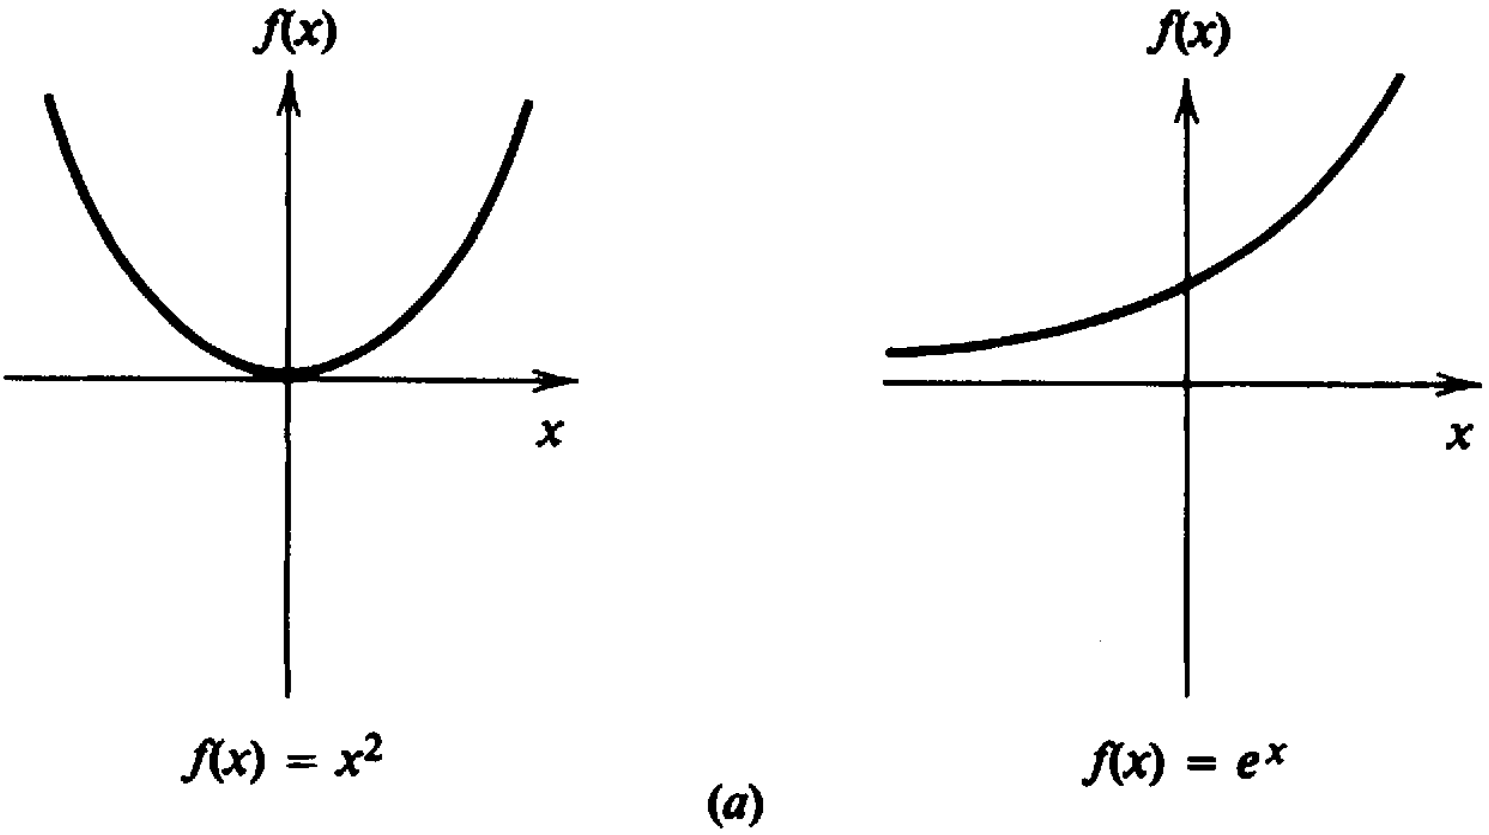
\includegraphics[width=\linewidth]{Figures/convex.png}
        \label{fig:fig1}
    \end{minipage}
    \hspace{0.05\textwidth} % horizontal space between the two figures
    % Second figure
    \begin{minipage}{0.45\textwidth}
        \centering
        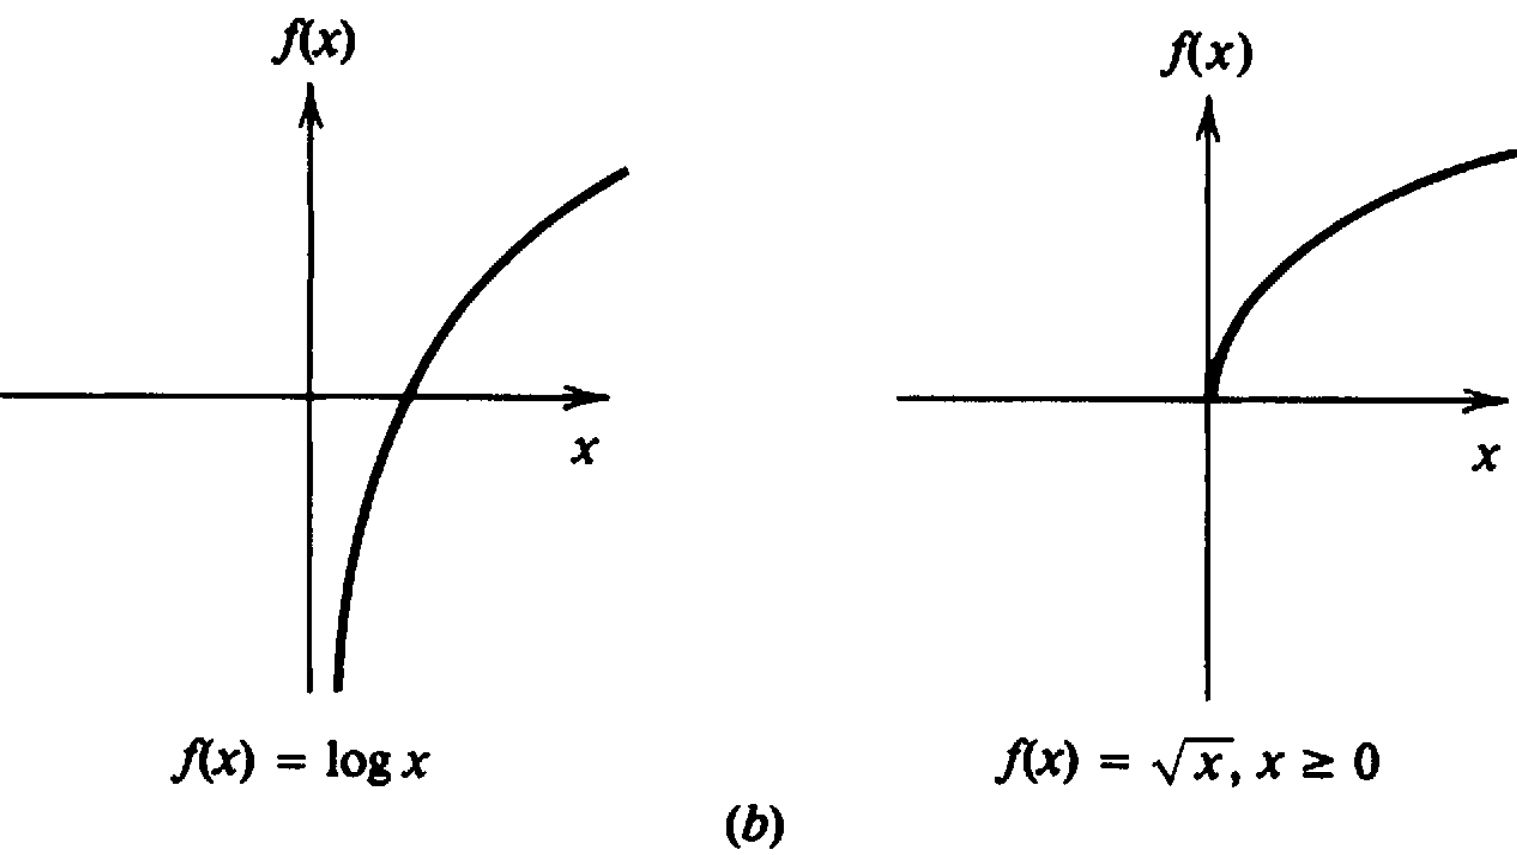
\includegraphics[width=\linewidth]{Figures/concave.png}
        \label{fig:fig2}
    \end{minipage}
    \caption{Examples of (a) convex and (b) concave functions.}
\end{figure}


\begin{infobox}[Geometric Interpretation]
    \begin{itemize}
        \item A function is \textbf{convex} if it always lies \textbf{below} any chord connecting two points on its graph
        \item A function is \textbf{concave} if it always lies \textbf{above} any chord connecting two points on its graph
        \item Linear functions \(ax + b\) are both convex and concave
    \end{itemize}
\end{infobox}

\subsection{Jensen's Inequality}

\begin{formulabox}[Theorem 2.6.2: Jensen's Inequality]
    If \(f\) is a convex function and \(X\) is a random variable, then:
    \[
        E[f(X)] \ge f(E[X])
    \]

    Moreover, if \(f\) is strictly convex, equality holds if and only if \(X = E[X]\) with probability 1.
\end{formulabox}

\begin{infobox}[Interpretation]
    \begin{itemize}
        \item For a convex function, the \textbf{expected value of the function} is at least as large as the \textbf{function of the expected value}.
        \item For a concave function (like \(\log\)), the inequality reverses:
              \[
                  E[f(X)] \le f(E[X])
              \]
        \item This is fundamental in proving properties of entropy and relative entropy.
    \end{itemize}
\end{infobox}

\subsection{Consequences of Jensen's Inequality}

\begin{formulabox}[Non-negativity of Relative Entropy: \(D(p \| q) \ge 0\)]
    For any two probability distributions \(p\) and \(q\):
    \[
        D(p \| q) = \sum_x p(x) \log \frac{p(x)}{q(x)} \ge 0
    \]
    Equality holds if and only if \(p(x) = q(x)\) for all \(x\).
\end{formulabox}

\begin{formulabox}[Non-negativity of Mutual Information: \(I(X;Y) \ge 0\)]
    For any two random variables \(X\) and \(Y\):
    \[
        I(X;Y) = D(p(x,y) \| p(x)p(y)) \ge 0
    \]
    Equality holds if and only if \(X\) and \(Y\) are independent.
\end{formulabox}

\begin{formulabox}[Conditioning Reduces Entropy: \(H(X|Y) \le H(X)\)]
    For any two random variables \(X\) and \(Y\):
    \[
        H(X|Y) \le H(X)
    \]
    Equality holds if and only if \(X\) and \(Y\) are independent.
\end{formulabox}

\begin{formulabox}[Independence Condition]
    For random variables \(X\) and \(Y\):
    \[
        H(X,Y) = H(X) + H(Y)
    \]
    if and only if \(X\) and \(Y\) are independent.
\end{formulabox}

\begin{infobox}[Interpretation]
    \begin{itemize}
        \item Knowing another random variable \(Y\) can only \textbf{reduce} (or leave unchanged) the uncertainty about \(X\).
        \item Mutual information and relative entropy are always non-negative because \(\log\) is concave, via Jensen's inequality.
        \item Independence occurs when knowledge of \(Y\) gives no information about \(X\), i.e., all inequalities become equalities.
    \end{itemize}
\end{infobox}

\chapter{Source Coding and Data Compression}

%==================================================
\section{Introduction to Source Coding}

\begin{definitionbox}[Source Coding]
\begin{itemize}
    \item Source coding is the process of \textbf{compressing data} to reduce redundancy
    while preserving the essential information.
    \item It is used to represent data efficiently for \textbf{transmission or storage}.
    \item The main objective is to \textbf{minimize the number of bits required}
    to encode source symbols \textbf{without losing information}.
\end{itemize}
\end{definitionbox}

%==================================================
\section{Data Compression -- Lossy vs Lossless}

$\rightarrow$ There are two main types of source coding techniques.

\begin{definitionbox}[Lossless Source Coding]
\begin{itemize}
    \item Lossless source coding ensures that the \textbf{original data can be perfectly
    reconstructed} from the compressed data.
    \item \textbf{Examples:} Huffman coding, Run-length coding, Arithmetic coding.
    \item \textbf{Use cases:} Text files, medical imaging, scientific data.
\end{itemize}
\end{definitionbox}

\begin{definitionbox}[Lossy Source Coding]
\begin{itemize}
    \item Lossy source coding reduces data size by \textbf{discarding less important
    information}, which may result in a loss of quality.
    \item \textbf{Examples:} JPEG (images), MP3 (audio), MPEG (video).
    \item \textbf{Use cases:} Multimedia applications where minor losses are acceptable.
\end{itemize}
\end{definitionbox}

%==================================================
\section{Compression Ratio}

\begin{formulabox}[Compression Ratio]
The compression ratio is defined as
\[
R = \frac{n_1}{n_2} > 1
\]
where
\[
n_1 = \text{size of uncompressed data}, \qquad
n_2 = \text{size of compressed data}.
\]
\end{formulabox}

%==================================================
\section{Redundancy}

\begin{definitionbox}[Redundancy]
Redundancy represents removable unnecessary data in a source.
\end{definitionbox}

\begin{formulabox}[Redundancy]
    \[
\text{Redundancy}
= \left(1 - \frac{1}{R}\right)\%
= \left(1 - \frac{n_2}{n_1}\right)\%
= \frac{n_1 - n_2}{n_1}\%
\]
\end{formulabox}

%==================================================
\section{Fixed-Length vs Variable-Length Coding}

\begin{definitionbox}[Fixed-Length Coding]
Every symbol is represented by the \textbf{same number of bits}.
\begin{itemize}
    \item Example: 3-bit code for 8 symbols.
    \item Simple but inefficient when symbol probabilities are unequal.
\end{itemize}
\end{definitionbox}

\begin{definitionbox}[Variable-Length Coding]
Different symbols are assigned codewords of \textbf{different lengths}.
\begin{itemize}
    \item More probable symbols get shorter codewords.
    \item Typical algorithms: Huffman coding, Arithmetic coding.
\end{itemize}
\end{definitionbox}

%==================================================
\section{Source Coding Theorem (Shannon's First Theorem)}

\begin{definitionbox}[Source Coding Theorem]
For a discrete memoryless source \(X\) with entropy \(H(X)\),
the average codeword length \(L\) of any distortionless source coding scheme satisfies
\[
H(X) \le L < H(X) + 1
\]

\begin{itemize}
    \item This gives the \textbf{best possible limit for lossless data compression}.
    \item Efficient schemes such as \textbf{Huffman coding} can achieve
    \(L \approx H(X)\) but cannot go below it.
\end{itemize}
\end{definitionbox}

%==================================================
\section{Coding Efficiency}

\begin{formulabox}[Coding Efficiency]
Coding efficiency measures how closely a coding scheme approaches the
theoretical limit set by entropy.

\[
\eta = \frac{H(X)}{L} \times 100\%
\]

The average codeword length is given by
\[
L = \sum_{i} p(x_i)\, l_i
\]

where
\begin{itemize}
    \item \(H(X)\): minimum average bits required per symbol (entropy),
    \item \(L\): actual average codeword length (bits per symbol),
    \item \(l_i\): length of the codeword for symbol \(x_i\),
    \item \(p(x_i)\): probability of symbol \(x_i\).
\end{itemize}

For a perfectly efficient coding scheme:
\[
L = H(X)
\]
\end{formulabox}


%==================================================
\section{Kraft--McMillan Inequality}

\begin{definitionbox}[Kraft--McMillan Inequality]
\begin{itemize}
    \item The Kraft--McMillan inequality provides a \textbf{necessary and sufficient condition}
    for the existence of a \textbf{binary uniquely decodable code}
    (and hence for a \textbf{binary prefix code}).
\end{itemize}

\begin{formulabox}[Kraft--McMillan Inequality]
    For codeword lengths
    \[
        n_1, n_2, \dots, n_L,
    \]
    a binary prefix (or uniquely decodable) code exists if and only if
    \[
        \sum_{k=1}^{L} 2^{-n_k} \le 1.
    \]
\end{formulabox}
    
\begin{itemize}
    \item If the inequality holds, a prefix code can be constructed.

    \item Equality implies an \textbf{optimally efficient code}
    (no unused code space).

    \item \textbf{Prefix code:} No codeword is a prefix of another codeword,
    which guarantees unique decodability.
\end{itemize}
\end{definitionbox}

\begin{questionanswerbox}
\label{ex:Construction_of_a_Binary_Prefix_Code_using_Kraft_Inequality}
\textbf{Example: Construction of a Binary Prefix Code using Kraft Inequality}

\medskip
\textbf{Q:} Consider a set of symbols \(\{A,B,C,D\}\) with codeword lengths: \(\{1,2,3,3\}\). Find the binary prefix code using Kraft Inequality.

\medskip
\textbf{A:}
\medskip\\
\textbf{Step 1: Apply Kraft--McMillan inequality}

For a binary prefix code, the Kraft inequality is:
\[
\sum_{k=1}^{L} 2^{-l_k} \le 1
\]

Substituting the given lengths:
\[
2^{-1} + 2^{-2} + 2^{-3} + 2^{-3}
= \frac{1}{2} + \frac{1}{4} + \frac{1}{8} + \frac{1}{8}
= 1
\]

Since
\[
\sum 2^{-l_k} = 1 \le 1,
\]
the Kraft inequality is satisfied.

\medskip
\textbf{Step 2: Construct the prefix code using a binary tree}

Because the Kraft inequality holds with equality, a
\textbf{binary prefix code can be constructed}.

\begin{figure}[H]
    \centering
    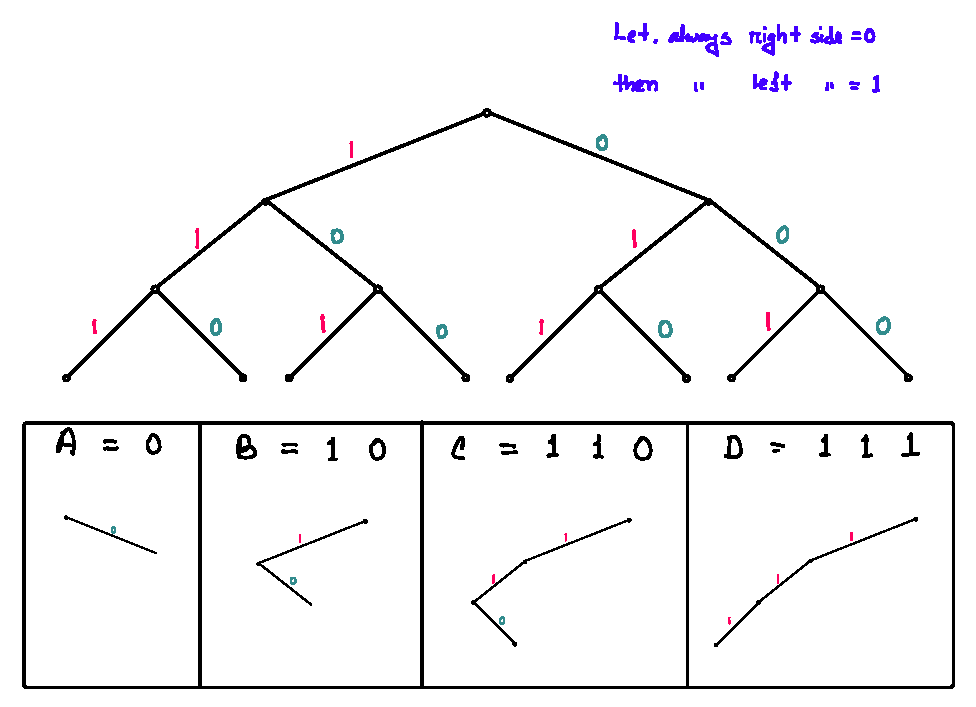
\includegraphics[width=0.9\linewidth]{Figures/Binary tree for the example.pdf}
    \caption{Binary tree for Example~\ref{ex:Construction_of_a_Binary_Prefix_Code_using_Kraft_Inequality}}
    \label{fig:binary_tree_kraft_example}
\end{figure}

So then one possible assignment is:
\[
A \rightarrow 0,\quad
B \rightarrow 10,\quad
C \rightarrow 110,\quad
D \rightarrow 111
\]

\textbf{Step 3: Interpretation}

The constructed code is:
\[
\{0,\;10,\;110,\;111\}
\]

No codeword is a prefix of another, hence the code is
\textbf{prefix-free and uniquely decodable}.

\medskip\\
\textbf{Conclusion:}
A valid \textbf{binary prefix code} exists for the given set of codeword lengths.
Since equality holds in Kraft’s inequality, the code is
\textbf{optimally efficient}.
\end{questionanswerbox}

\begin{questionanswerbox}
\textbf{Q:}  
Check whether a prefix code exists for codeword lengths
\[
\{1,\,2,\,3,\,3\}.
\]
\medskip
\textbf{A:}
\[
\sum_{k=1}^{4} 2^{-n_k}
=2^{-1}+2^{-2}+2^{-3}+2^{-3}
=1
\]

Since the inequality is satisfied, a prefix code exists.

\medskip
One possible prefix code is:

\begin{center}
\renewcommand{\arraystretch}{1.4}
\setlength{\tabcolsep}{10pt}
\begin{tabular}{|c|c|c|}
\hline
\textbf{Symbol} & \textbf{Codeword} & \textbf{Length} \\
\hline
\(a\) & 0   & 1 \\
\(b\) & 10  & 2 \\
\(c\) & 110 & 3 \\
\(d\) & 111 & 3 \\
\hline
\end{tabular}
\end{center}

\medskip
Resulting prefix code:
\[
\{0,\;10,\;110,\;111\}
\]
\end{questionanswerbox}

\begin{formulabox}[Shannon Codeword Length]
For a source symbol \(x_i\) with probability \(p(x_i)\), the Shannon codeword
length is defined as:
\[
l_i = \left\lceil \log_2 \frac{1}{p(x_i)} \right\rceil
\]

This represents the \textbf{minimum number of bits} required to encode the symbol
based on its probability.
\end{formulabox}

\section{Shannon--Fano--Elias Coding}

\begin{definitionbox}[Shannon--Fano--Elias Coding]
\begin{itemize}
    \item Shannon--Fano--Elias (SFE) coding is a \textbf{prefix coding technique}
    used in information theory to assign binary codewords based on symbol probabilities.
    \item Codewords are generated using the \textbf{cumulative distribution function (CDF)}
    of the source symbols.
    \item The generated code is \textbf{prefix-free} and hence
    \textbf{uniquely decodable}.
    \item Codeword lengths are chosen based on symbol probabilities and
    satisfy the \textbf{Kraft--McMillan inequality}.
\end{itemize}
\end{definitionbox}

%--------------------------------------------------
\begin{infobox}[Procedure for Shannon--Fano--Elias Coding]
\begin{enumerate}
    \item Compute symbol probabilities \(p(x_i)\).
    \item Compute the cumulative distribution function:
    \[
        F(x_i)=\sum_{k<i} p(x_k)
    \]
    \item Compute the center (midpoint) value:
    \[
        \bar{F}(x_i)=\sum_{k<i} p(x_k)+\frac{1}{2}p(x_i)
    \]
    \item Assign binary codewords using the binary expansion of \(\bar{F}(x_i)\),
    with codeword length
    \[
        l_i=\left\lceil \log_2\frac{1}{p(x_i)} \right\rceil + 1
    \]
\end{enumerate}
\end{infobox}

%==================================================
\section{Shannon--Fano Coding}

\begin{definitionbox}[Shannon--Fano Coding]
\begin{itemize}
    \item Shannon--Fano coding is a \textbf{lossless source coding technique}.
    \item Binary codewords are assigned to symbols based on their probabilities.
    \item The objective is to construct a \textbf{prefix-free code}
    with \textbf{near-minimum average codeword length}.
\end{itemize}
\end{definitionbox}

%--------------------------------------------------
\begin{infobox}[Steps in Shannon--Fano Coding]
\begin{enumerate}
    \item Arrange symbols in \textbf{decreasing order of probability}.
    \item Split the list into two parts with \textbf{nearly equal total probability}.
    \item Assign \texttt{0} to the first group and \texttt{1} to the second group.
    \item Recursively apply the same procedure to each group
    until each symbol is assigned a codeword.
\end{enumerate}
\end{infobox}

%==================================================
\begin{infobox}[Key Difference: Shannon--Fano vs Shannon--Fano--Elias]
\begin{itemize}
    \item \textbf{Shannon--Fano coding} uses \textbf{recursive probability splitting}.
    \item \textbf{Shannon--Fano--Elias coding} uses the \textbf{cumulative distribution function}.
    \item Both generate \textbf{prefix-free} and \textbf{uniquely decodable} codes.
\end{itemize}
\end{infobox}

\begin{questionanswerbox}
\textbf{Q:}
Find the codewords occurring for the probability set
\[
\left\{\tfrac12,\;\tfrac14,\;\tfrac18,\;\tfrac18\right\}
\]
for symbols \(s_1,s_2,s_3,s_4\). Find efficiency and redundancy.

\medskip\\
\textbf{A:}

\medskip
\textbf{Given:}
\[
p(s_1)=\tfrac12,\quad
p(s_2)=\tfrac14,\quad
p(s_3)=\tfrac18,\quad
p(s_4)=\tfrac18.
\]

\medskip
\textbf{Step 1: Shannon--Fano construction (bracket method):}
\begin{enumerate}[label=\textbf{\roman*}.]
    \item \textbf{Arrange symbols in decreasing order of probability:}

        \[
        \begin{array}{l}
        s_1\;(1/2)\\
        s_2\;(1/4)\\
        s_3\;(1/8)\\
        s_4\;(1/8)
        \end{array}
        \]
    \item \textbf{First split (assign 0 and 1)}
        \[
        \begin{aligned}
        \left.
        \begin{array}{l}
        s_1\,(1/2)
        \end{array}
        \right\}
        &\xrightarrow{\tfrac12}\;0 \\[10pt]
        \left.
        \begin{array}{l}
        s_2\,(1/4)\\
        s_3\,(1/8)\\
        s_4\,(1/8)
        \end{array}
        \right\}
        &\xrightarrow{\tfrac12}\;1
        \end{aligned}
        \]
    \item \textbf{Second split (assign 10 and 11)}
        \[
        \begin{aligned}
        \left.
        \begin{array}{l}
        s_2\,(1/4)
        \end{array}
        \right\}
        &\xrightarrow{\tfrac14}\;10 \\[10pt]
        \left.
        \begin{array}{l}
        s_3\,(1/8)\\
        s_4\,(1/8)
        \end{array}
        \right\}
        &\xrightarrow{\tfrac14}\;11
        \end{aligned}
        \]
    \item \textbf{Final split}
        \[
        \begin{aligned}
        s_3\,(1/8) &\xrightarrow{\tfrac18}\;110 \\[8pt]
        s_4\,(1/8) &\xrightarrow{\tfrac18}\;111
        \end{aligned}
        \]
\end{enumerate}

\textbf{Shannon--Fano code construction (one valid assignment)}

\renewcommand{\arraystretch}{1.4}
\setlength{\tabcolsep}{6pt}
\newcolumntype{C}[1]{>{\centering\arraybackslash}m{#1}}

\begin{longtable}{|C{1.6cm}|C{2.2cm}|C{1.6cm}|C{1.6cm}|C{1.6cm}|C{2.2cm}|C{1.6cm}|}
\hline
\rowcolor{gray!20}
\textbf{Symbol} & \textbf{Probability} & \multicolumn{3}{c|}{\textbf{Process}} & \textbf{Codeword} & \textbf{Length} \\
\hline
\endhead

\(s_1\) & \(\tfrac12\) & \multicolumn{3}{c|}{0} & 0 & 1 \\
\hline

\(s_2\) & \(\tfrac14\)
& \multirow{3}{*}{\(\mathbf{1}\)}
& \multicolumn{2}{c|}{0}
& 10 & 2 \\
\cline{1-2}\cline{4-7}

\(s_3\) & \(\tfrac18\)
&
& \multirow{2}{*}{1}
& 0
& 110 & 3 \\
\cline{1-2}\cline{5-7}

\(s_4\) & \(\tfrac18\)
&
&
& 1
& 111 & 3 \\
\hline

\caption{Shannon--Fano construction shown inside the table (merged Process cells)}
\label{tab:sf_process_merged}
\end{longtable}

\textbf{Step 2: Entropy of the source}
\begin{align*}
H(X)
&= -\sum_{i=1}^{4} p(s_i)\log_2 p(s_i)\\[4pt]
&= -\Big[
\tfrac12\log_2\!\big(\tfrac12\big)
+\tfrac14\log_2\!\big(\tfrac14\big)
+\tfrac18\log_2\!\big(\tfrac18\big)
+\tfrac18\log_2\!\big(\tfrac18\big)
\Big]\\[6pt]
&=\tfrac12\log_2 2
+\tfrac14\log_2 4
+\tfrac18\log_2 8
+\tfrac18\log_2 8\\[4pt]
&= 1.75\ \text{bits/symbol}.
\end{align*}

\medskip
\textbf{Step 3: Average codeword length}

\begin{align*}
L
&=\sum_{i=1}^{4} p(s_i)\,l_i\\[4pt]
&=(1)\!\left(\tfrac12\right)
+(2)\!\left(\tfrac14\right)
+(3)\!\left(\tfrac18\right)
+(3)\!\left(\tfrac18\right)\\[4pt]
&= 1.75\ \text{bits/symbol}.
\end{align*}

\medskip
\textbf{Step 4: Coding efficiency and redundancy}

\[
\eta=\frac{H(X)}{L}\times 100\%
=\frac{1.75}{1.75}\times 100\%
=100\%.
\]

\[
R_e = 1-\eta = 1-1 = 0.
\]

\medskip
\textbf{Answer:}
\[
\boxed{\eta=100\%,\qquad R_e=0.}
\]
\end{questionanswerbox}

\section{Huffman Coding}
\begin{definitionbox}[Huffman Coding]
    A \textbf{variable-length prefix code}.
    Shorter codewords are assigned to the most probable symbols.
    The same tree is needed both for encoding and decoding.
\end{definitionbox}

\begin{infobox}[Prefix Property]
    No codeword is a prefix of any other codeword, guaranteeing instantaneous
    decodability.
\end{infobox}

\begin{questionanswerbox}
    \label{ex:huffman_example1} % <-- Label for referencing this example
    \textbf{Q: Example 1} (probabilities in descending order)

    \[
        P(a)=0.3,\; P(b)=0.3,\; P(c)=0.233,\; P(d)=0.167,\; P(e)=0.067
    \]

    \textbf{A:}
    \begin{enumerate}
        \item Combine the two smallest probabilities (\(e\) and \(d\)) to form a node of probability \(0.167 + 0.067 = 0.234\).
        \item Repeat merging until a single root of probability 1 is obtained.
    \end{enumerate}

    The resulting \textbf{Huffman tree} yields the codewords:

    \begin{center}
        \renewcommand{\arraystretch}{1.2}
        \setlength{\tabcolsep}{10pt}

        \begin{longtable}{|c|c|}
            \hline
            \rowcolor{gray!25}
            \textbf{Symbol} & \textbf{Code} \\
            \hline
            \endfirsthead

            \hline
            \rowcolor{gray!25}
            \textbf{Symbol} & \textbf{Code} \\
            \hline
            \endhead

            a               & 0             \\
            b               & 10            \\
            c               & 110           \\
            d               & 1111          \\
            e               & 1110          \\
            \hline
            \caption{Symbol-Code Mapping for Example~\ref{ex:huffman_example1}}
            \label{tab:huffman_symbol_code_ex1}
        \end{longtable}

    \end{center}

    \textbf{Decoding Example} (bit-stream: \texttt{10 1110 110 0})

    \begin{itemize}
        \item Start from right to left.
        \item \texttt{0} $\to$ symbol \texttt{a}
        \item \texttt{110} $\to$ 1 $\to$ 1 $\to$ 0 $\to$ symbol \texttt{c}
        \item \texttt{1110} $\to$ 1 $\to$ 1 $\to$ 1 $\to$ 0 $\to$ symbol \texttt{d}
        \item \texttt{10} $\to$ 1 $\to$ 0 $\to$ symbol \texttt{b}
    \end{itemize}

    \[
        \therefore \text{Decoded message: } \texttt{b d c a}
    \]

    % Optional: Add tree image if available
    \begin{figure}[H]
        \centering
        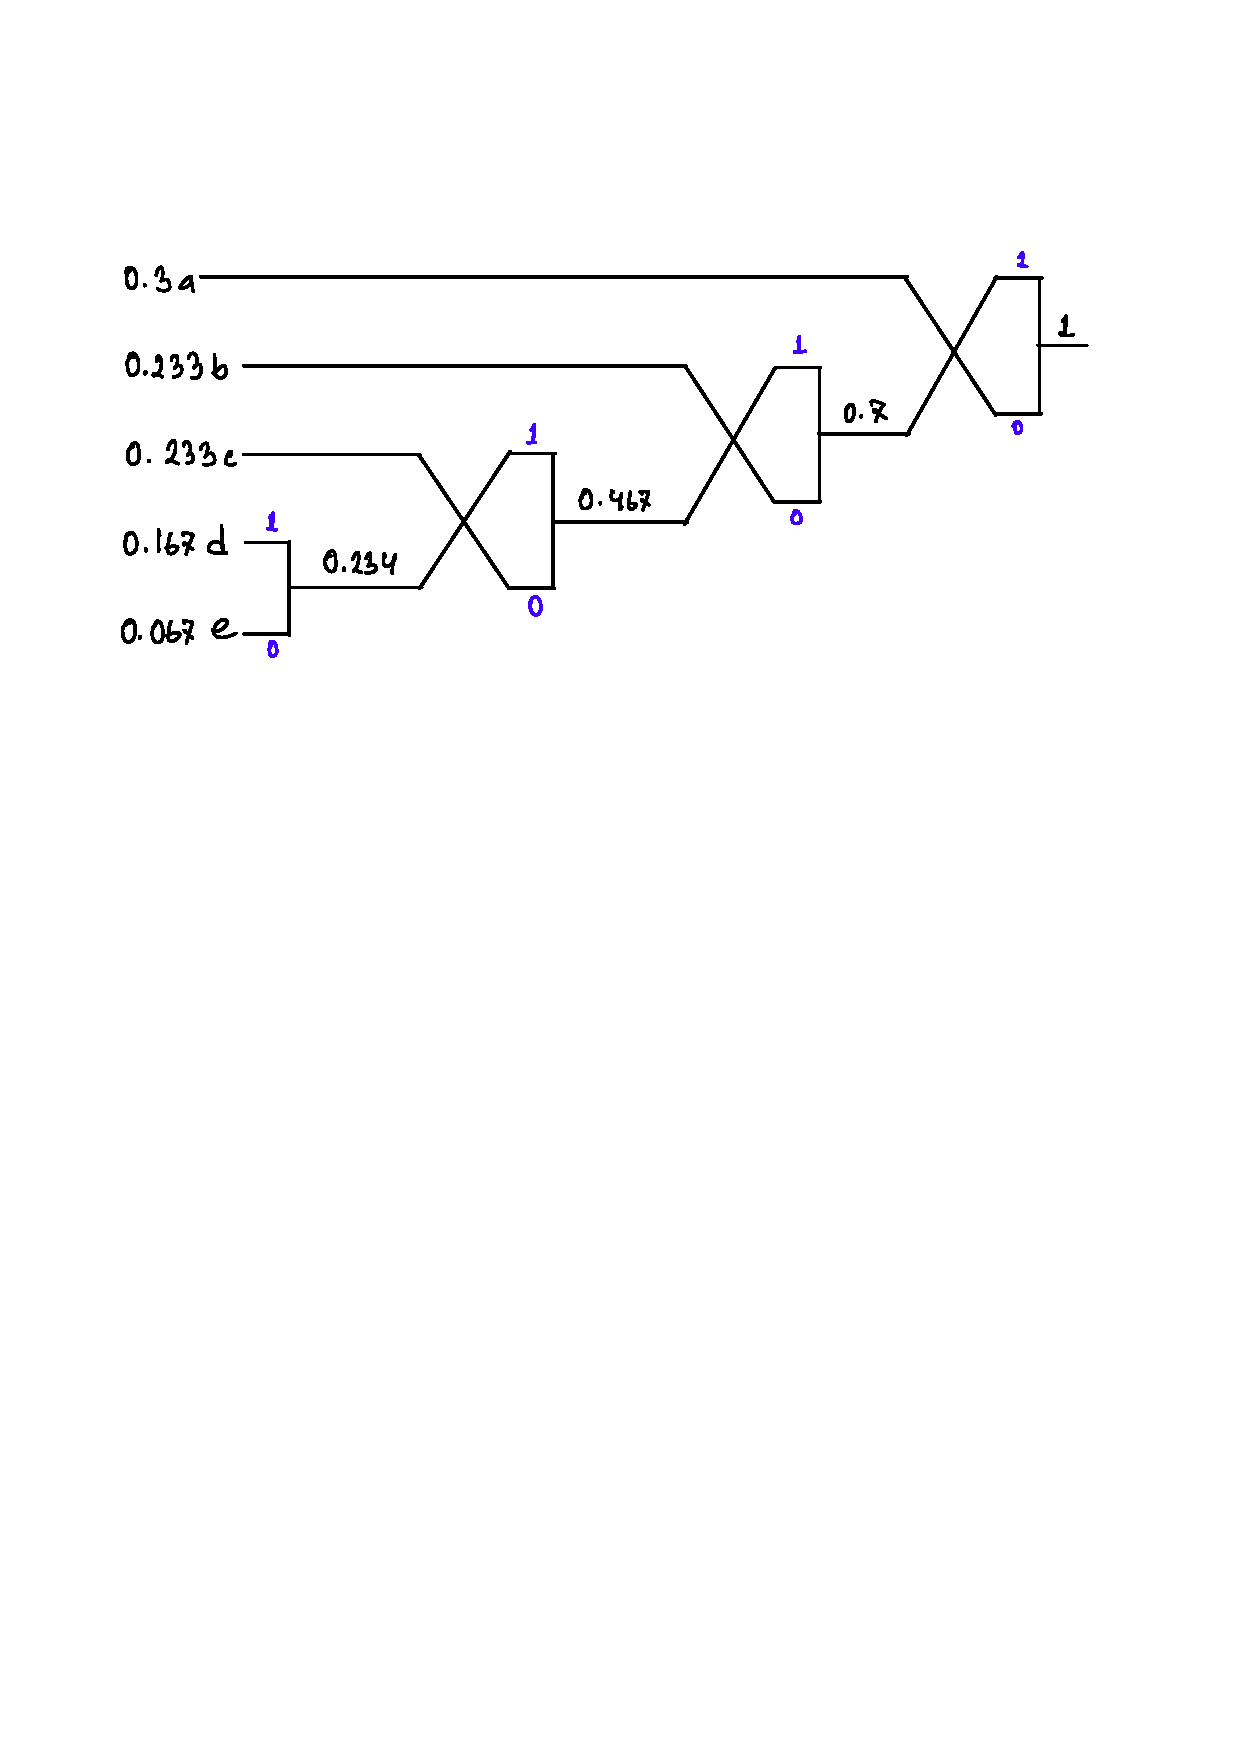
\includegraphics[width=0.9\linewidth]{Figures/huffman_tree_example1.pdf}
        \caption{Huffman tree for Example~\ref{ex:huffman_example1}}
        \label{fig:huffman_tree_ex1}
    \end{figure}

\end{questionanswerbox}

\begin{questionanswerbox}
    \label{ex:huffman_example2}
    \textbf{Example 2}

    \[
        P(a)=0.6,\; P(b)=0.15,\; P(c)=0.1,\; P(d)=0.075,\; P(e)=0.05,\; P(f)=0.025
    \]

    \begin{figure}[H]
        \centering
        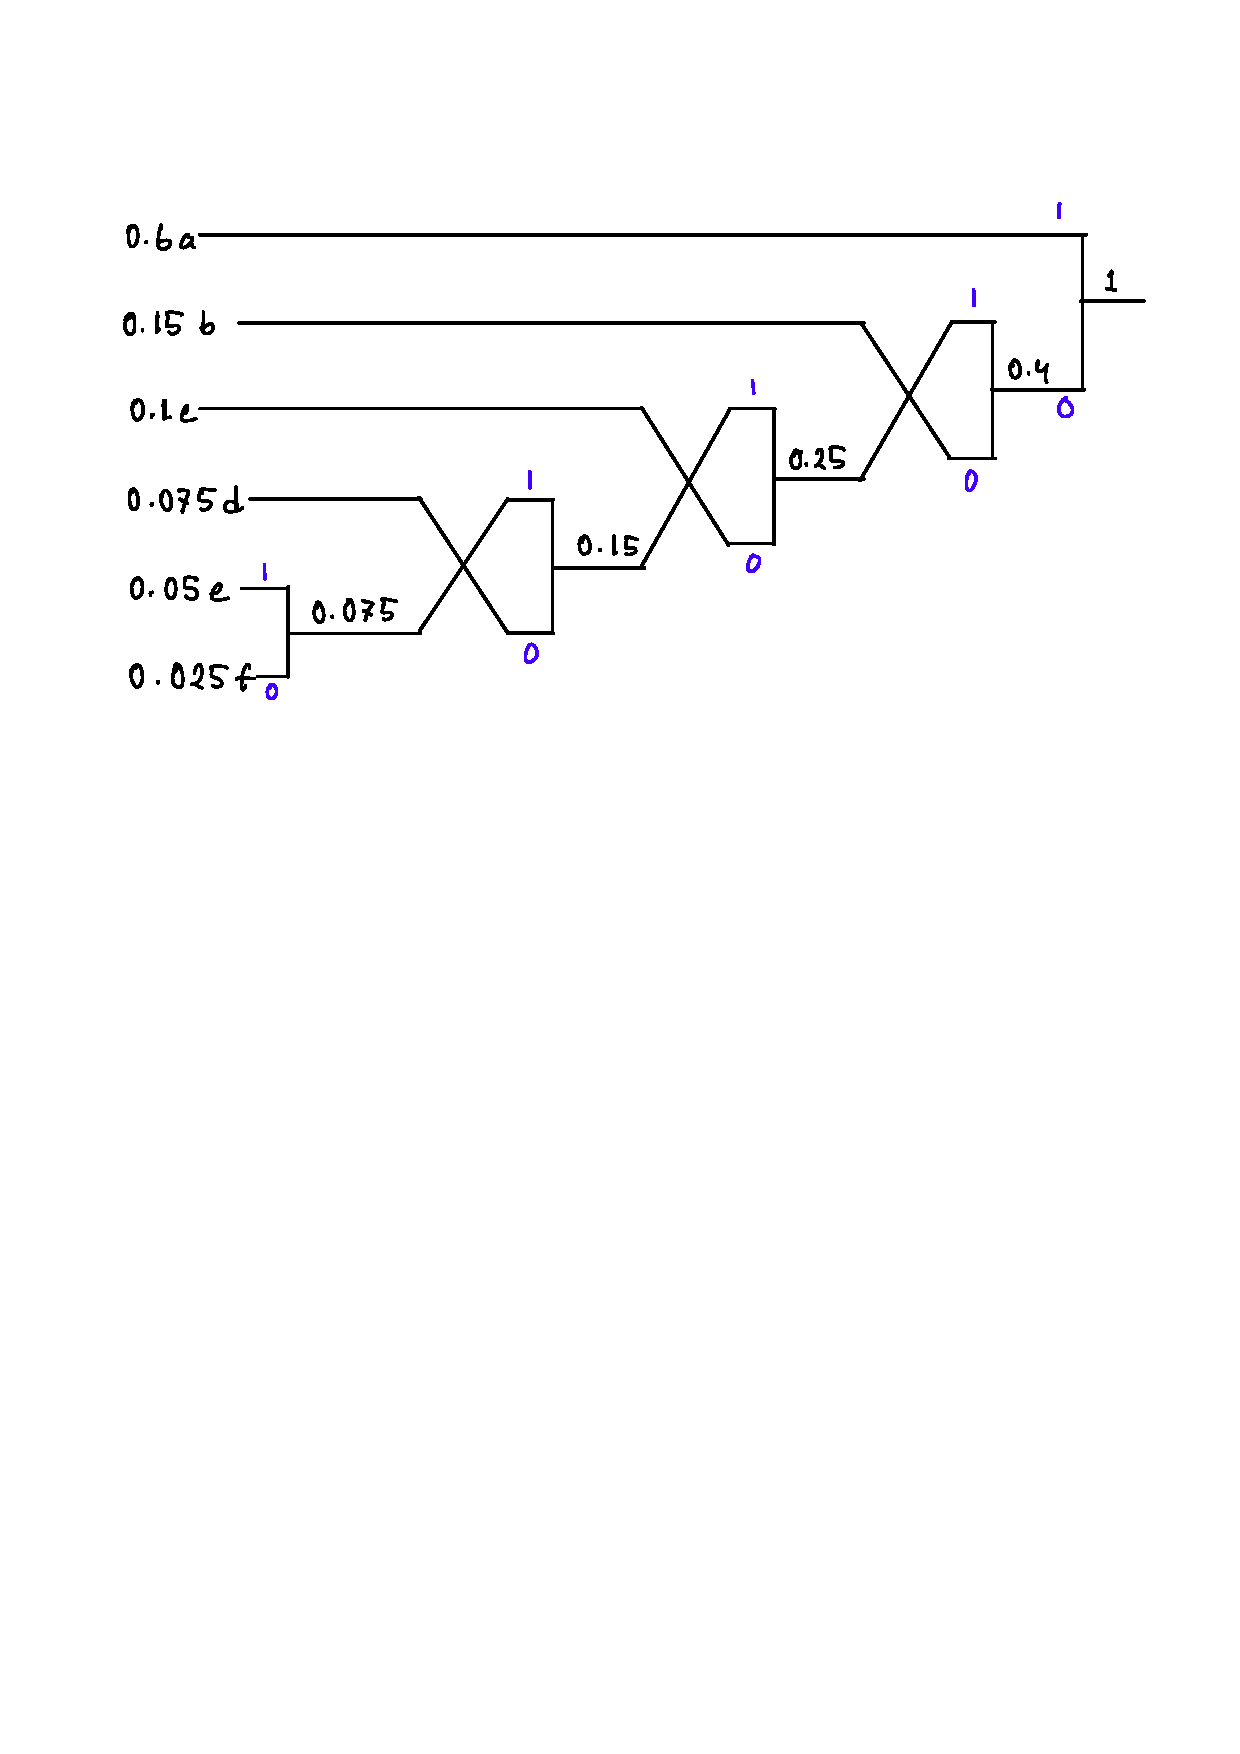
\includegraphics[width=0.9\linewidth]{Figures/huffman_tree_example2.pdf}
        \caption{Huffman tree for Example~\ref{ex:huffman_example2}}
        \label{fig:huffman_ex1}
    \end{figure}

    The tree (root to probability 1) produces:

    \begin{center}
        \renewcommand{\arraystretch}{1.2}
        \setlength{\tabcolsep}{8pt}

        \begin{longtable}{|c|c|}
            \hline
            \rowcolor{gray!25}
            \textbf{Symbol} & \textbf{Code} \\
            \hline
            \endfirsthead

            \hline
            \rowcolor{gray!25}
            \textbf{Symbol} & \textbf{Code} \\
            \hline
            \endhead

            a               & 1             \\
            b               & 00            \\
            c               & 010           \\
            d               & 0110          \\
            e               & 01111         \\
            f               & 01110         \\
            \hline
            \caption{Symbol-to-Code Mapping for Example~\ref{ex:huffman_example2}}
            \label{tab:symbol_code}
        \end{longtable}
    \end{center}
    \textbf{Decoding a stream}

    Bit-stream: \texttt{1 01110 1 1 00} to symbols \texttt{a f a a b}
\end{questionanswerbox}

\section{Efficiency of Huffman Coding}
\begin{formulabox}[Efficiency]
    \[
        \eta = \frac{H(X)}{\bar{R}}
    \]

    \begin{itemize}
        \item Entropy
              \[
                  H(X)=-\sum_{k} p(x_k)\log_2 p(x_k)
              \]
        \item Average codeword length
              \[
                  \bar{R}=\sum_{k} n_k p(x_k)\qquad (n_k=\text{bits of symbol }k)
              \]
    \end{itemize}
\end{formulabox}

\section{Arithmetic Coding}
\begin{definitionbox}[Arithmetic Coding]
    \begin{itemize}
        \item Encodes an \textbf{entire message} into a \textbf{single fractional number} between 0 and 1 that lies inside a unique interval.
        \item Each symbol narrows the current interval based on its probability.
    \end{itemize}
\end{definitionbox}

\begin{formulabox}[Interval Update Rule]
    For the \(k\)-th symbol with probability \(P\):

    \[
        \begin{aligned}
            \text{Upper limit of new interval} & = (\text{D} \times P) + \text{Lower limit of new interval} \\
            \text{Lower limit of new interval} & = \text{Upper limit of previous interval}
        \end{aligned}
    \]

    Let:
    \begin{itemize}
        \item \(D\) = Total difference
        \item \(P\) = Probability
    \end{itemize}
\end{formulabox}

\begin{questionanswerbox}
    \label{ex:arithmetic_coding_example1}
    \textbf{Example 1}

    \[
        P(a)=0.4,\quad P(b)=0.3,\quad P(c)=0.2,\quad P(d)=0.1
    \]

    Message: \texttt{b c d a}. Find the arithmetic code

    \textbf{A:}

    \begin{itemize}
        \item We build cumulative probability ranges:
              \begin{center}
                  \renewcommand{\arraystretch}{1.2}
                  \setlength{\tabcolsep}{10pt}

                  \begin{longtable}{|c|c|c|}
                      \hline
                      \rowcolor{gray!25}
                      \textbf{Symbol} & \textbf{Width} & \textbf{Range}             \\
                      \hline
                      \endfirsthead

                      \hline
                      \rowcolor{gray!25}
                      \textbf{Symbol} & \textbf{Width} & \textbf{Range}             \\
                      \hline
                      \endhead

                      d               & 0.1            & $[0.0, (0.0 + 0.1) = 0.1)$ \\
                      c               & 0.2            & $[0.1, (0.1 + 0.2) = 0.3)$ \\
                      b               & 0.3            & $[0.3, (0.3 + 0.3) = 0.6)$ \\
                      a               & 0.4            & $[0.6, (0.6 + 0.4) = 1.0)$ \\
                      \hline
                      \caption{Symbol-Width-Range Mapping for Example \ref{ex:arithmetic_coding_example1}}
                      \label{tab:symbol_width_range}
                  \end{longtable}
              \end{center}
        \item \textbf{Step-by-step encoding}:

              \begin{enumerate}
                  \item \textbf{Symbol b} (initially: range $[0.3,0.6)$)
                        \begin{itemize}
                            \item Current interval: $L=0.3,\; U=0.6,\; D=U-L=0.3$.
                            \item Subintervals inside $[0.3,0.6)$ (widths scaled by $D=0.3$):
                                  \[
                                      \begin{aligned}
                                          \text{d} & : {[0.300,\;0.300 + 0.3\times0.1)} = {[0.300,\;0.330)} \\
                                          \text{c} & : {[0.330,\;0.330 + 0.3\times0.2)} = {[0.330,\;0.390)} \\
                                          \text{b} & : {[0.390,\;0.390 + 0.3\times0.3)} = {[0.390,\;0.480)} \\
                                          \text{a} & : {[0.480,\;0.480 + 0.3\times0.4)} = {[0.480,\;0.600)}
                                      \end{aligned}
                                  \]
                        \end{itemize}

                  \item \textbf{Symbol c} (now: range of interest $[0.330,0.390)$)
                        \begin{itemize}
                            \item Current interval: $L=0.330,\; U=0.390,\; D=U-L=0.060$.
                            \item Subintervals inside $[0.330,0.390)$ (widths scaled by $D=0.060$):
                                  \[
                                      \begin{aligned}
                                          \text{d} & : {[0.330,\;0.330 + 0.060\times0.1)} = {[0.330,\;0.336)} \\
                                          \text{c} & : {[0.336,\;0.336 + 0.060\times0.2)} = {[0.336,\;0.348)} \\
                                          \text{b} & : {[0.348,\;0.348 + 0.060\times0.3)} = {[0.348,\;0.366)} \\
                                          \text{a} & : {[0.366,\;0.366 + 0.060\times0.4)} = {[0.366,\;0.390)}
                                      \end{aligned}
                                  \]
                        \end{itemize}

                  \item \textbf{Symbol d} (now: range of interest $[0.330,0.336)$)
                        \begin{itemize}
                            \item Current interval: $L=0.330,\; U=0.336,\; D=U-L=0.006$.
                            \item Subintervals inside $[0.330,0.336)$ (widths scaled by $D=0.006$):
                                  \[
                                      \begin{aligned}
                                          \text{d} & : {[0.330,\;0.330 + 0.006\times0.1)} = {[0.330,\;0.3306)}    \\
                                          \text{c} & : {[0.3306,\;0.3306 + 0.006\times0.2)} = {[0.3306,\;0.3318)} \\
                                          \text{b} & : {[0.3318,\;0.3318 + 0.006\times0.3)} = {[0.3318,\;0.3336)} \\
                                          \text{a} & : {[0.3336,\;0.3336 + 0.006\times0.4)} = {[0.3336,\;0.3360)}
                                      \end{aligned}
                                  \]
                        \end{itemize}

                  \item \textbf{Symbol a} (now: range of interest $[0.3336,0.3360)$)
                        \begin{itemize}
                            \item The true encoded value can be any number inside this interval
                            \item Every number inside this interval will correctly decode to the same original message
                            \item So both 0.334, 0.335, or 0.3359 would decode back to bcda
                        \end{itemize}
              \end{enumerate}
        \item \textbf{Final interval}: \([0.3336, 0.336)\)
        \item  \textbf{Tag}: Choose any number in final interval $\rightarrow$ e.g., $\mathbf{0.336}$
        \item The message \texttt{bcda} is encoded as the \textbf{single number}
              \[
                  \boxed{0.336}
              \]
        \item To convert the decimal fraction \(0.336_{10}\) into binary, multiply repeatedly by 2
              and record the integer part at each step.

              \renewcommand{\arraystretch}{1.3}
              \setlength{\tabcolsep}{5pt}

              % Custom column alignment
              \newcolumntype{C}[1]{>{\centering\arraybackslash}m{#1}}
              \newcolumntype{L}[1]{>{\raggedright\arraybackslash}m{#1}}

              \begin{longtable}{|C{1.2cm}|C{4.5cm}|C{2cm}|C{2.5cm}|}
                  \hline
                  \rowcolor{gray!25}
                  \textbf{Step} & \textbf{Operation}         & \textbf{Integer Part} & \textbf{Fraction Remaining} \tabularnewline
                  \hline
                  1             & \(0.336 \times 2 = 0.672\) & 0                     & 0.672                                       \\
                  \hline
                  2             & \(0.672 \times 2 = 1.344\) & 1                     & 0.344                                       \\
                  \hline
                  3             & \(0.344 \times 2 = 0.688\) & 0                     & 0.688                                       \\
                  \hline
                  4             & \(0.688 \times 2 = 1.376\) & 1                     & 0.376                                       \\
                  \hline
                  5             & \(0.376 \times 2 = 0.752\) & 0                     & 0.752                                       \\
                  \hline
                  6             & \(0.752 \times 2 = 1.504\) & 1                     & 0.504                                       \\
                  \hline
                  7             & \(0.504 \times 2 = 1.008\) & 1                     & 0.008                                       \\
                  \hline
                  \caption{Binary Conversion of \(0.336_{10}\) Using Multiply-by-2 Method}
                  \label{tab:binary_conversion_0336}
              \end{longtable}
              \[
                  \therefore 0.336_{10} \approx 0.0101011_2
              \]

              Thus, the binary equivalent of the message is:
              \[
                  \text{Message: bcda} \rightarrow \text{Tag: } 0.336 \rightarrow \text{Binary: } 0.01010112
              \]
    \end{itemize}

    \begin{figure}[H]
        \centering
        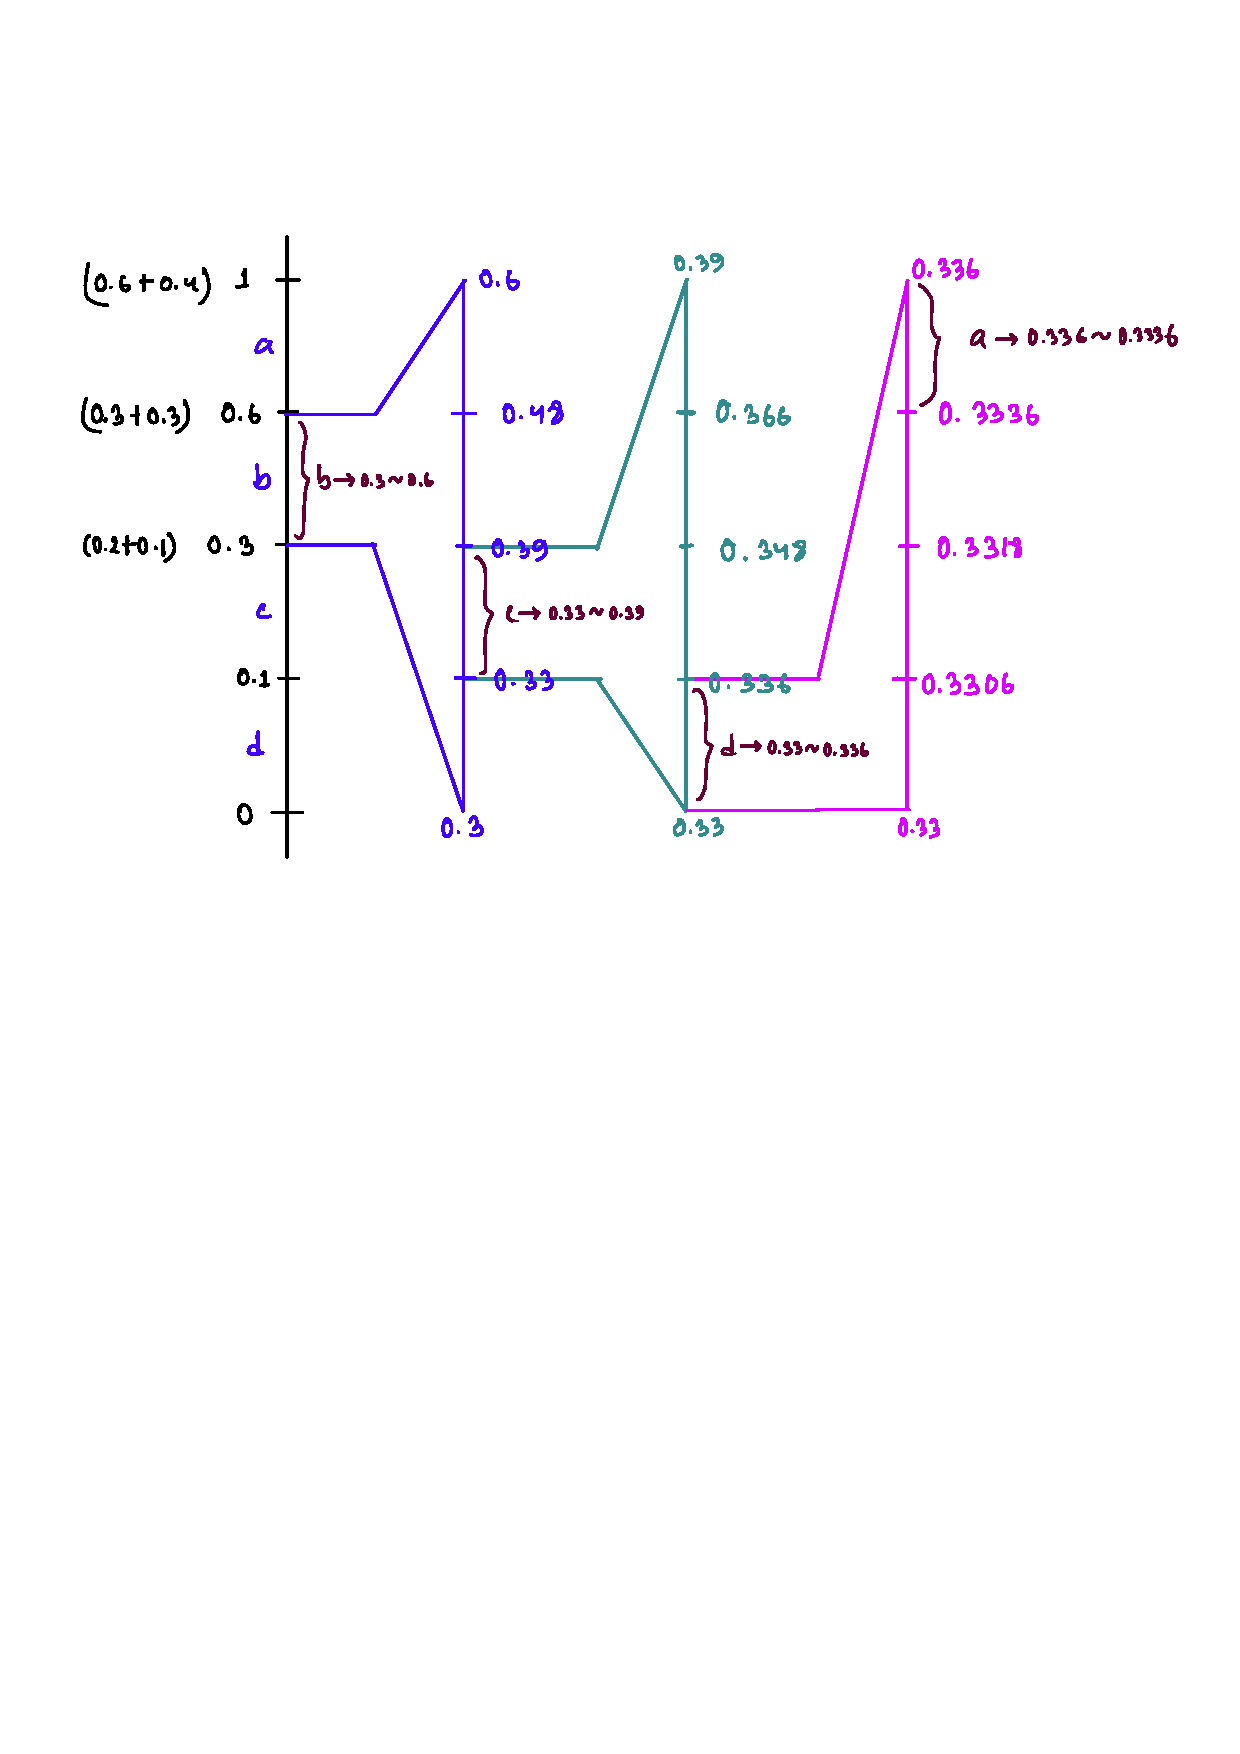
\includegraphics[width=0.95\linewidth]{Figures/arithmetic_coding_bcda.pdf}
        \caption{Arithmetic coding intervals for message \texttt{bcda}}
        \label{fig:arith_bcda}
    \end{figure}

\end{questionanswerbox}

\section{Run-Length Coding}
\begin{definitionbox}[Run-Length Coding]
    A \textbf{run} is a sequence of identical symbols.
    Run-length coding replaces each run by the pair (symbol, count).
\end{definitionbox}

\begin{questionanswerbox}
    Original: \texttt{a a b c a a a b c c c c c d d d} (16 symbols)

    Compressed: \texttt{(a,2)(b,1)(c,1)(a,3)(b,1)(c,5)(d,3)} (14 entries)

    Assuming 8 bits per entry:

    \[
        \text{Original}=16\times8=128\;\text{bits},\quad
        \text{Compressed}=14\times8=112\;\text{bits}
    \]
\end{questionanswerbox}

\chapter{Channel Coding}
\section{Overview of the Digital Communication System}
The digital communication system is comprised of multiple stages that work together to ensure efficient data transmission in the presence of noise and interference.

\begin{figure}[H]
    \centering
    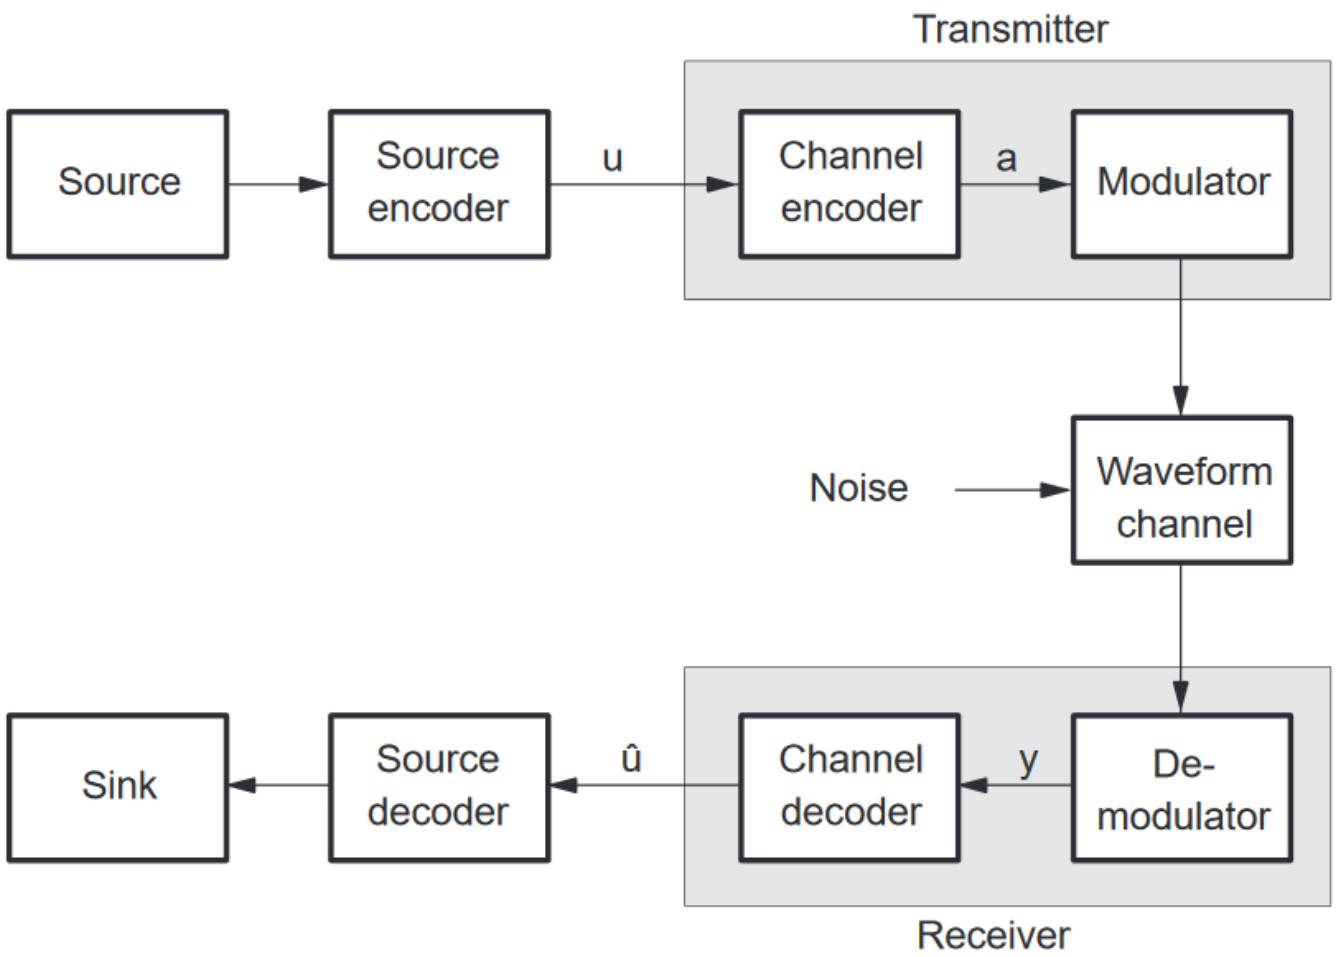
\includegraphics[width=0.6\linewidth]{Figures/Digital communication system.png}
    \caption{Digital Communication System}
    \label{fig:Digitalcommunicationsystem}
\end{figure}

\section{Data Flow in a Digital System}
Data flows through the following blocks in a typical digital communication system:

\begin{itemize}
    \item \textbf{Source Encoder:}
          \begin{itemize}
              \item Removes redundancy and compresses the input data.
              \item Converts the original data into a compact binary format for efficient transmission.
              \item Can perform either \textbf{lossless} or \textbf{lossy} compression depending on the application.
              \item Uses techniques such as \textbf{run-length coding}, \textbf{Huffman coding} (lossless), and \textbf{JPEG} (lossy).
          \end{itemize}

    \item \textbf{Channel Encoder:}
          \begin{itemize}
              \item Adds redundancy to the data to detect and correct errors that occur during transmission.
              \item Channel coding techniques help the system recover from noise and other impairments.
              \item Examples include \textbf{Hamming code}, \textbf{Reed-Solomon}, and \textbf{Turbo codes}.
          \end{itemize}

    \item \textbf{Modulator:}
          \begin{itemize}
              \item Modulates the encoded signal onto a carrier wave for transmission.
              \item Modulation schemes may include \textbf{Amplitude Modulation (AM)}, \textbf{Frequency Modulation (FM)}, and \textbf{Phase Modulation (PM)}.
          \end{itemize}

    \item \textbf{Channel:}
          \begin{itemize}
              \item The medium over which the signal is transmitted (e.g., air, fiber optic cables, or copper wires).
              \item The channel introduces noise, interference, and attenuation.
              \item Two types of channels:
                    \begin{itemize}
                        \item \textbf{Guided:} Includes wired communication (e.g., coaxial cables).
                        \item \textbf{Unguided:} Includes wireless communication (e.g., radio waves).
                    \end{itemize}
          \end{itemize}

    \item \textbf{Demodulator:}
          \begin{itemize}
              \item Demodulates the received signal to extract the encoded data.
              \item Performs the reverse operation of modulation.
          \end{itemize}

    \item \textbf{Channel Decoder:}
          \begin{itemize}
              \item Removes the redundancy added during channel encoding.
              \item Corrects any errors caused by noise in the channel.
          \end{itemize}

    \item \textbf{Source Decoder:}
          \begin{itemize}
              \item Converts the binary data back into its original form.
              \item Performs the reverse operation of source encoding.
              \item May involve decompression (e.g., decoding JPEG images or decompressing Huffman codes).
          \end{itemize}
\end{itemize}

\section{Importance of Channel Coding}

\begin{infobox}[Channel coding]
    Channel coding is essential because the communication channel often introduces noise, which can distort or corrupt the transmitted signal. To ensure that the original data can still be recovered, channel coding applies mathematical techniques that make the transmission more reliable.
\end{infobox}

\subsection{Why Noise Occurs in Channels}

\begin{itemize}[label=$\rightarrow$]
    \item Communication channels are generally of two types:
          \begin{itemize}
              \item \textbf{Guided channels}
              \item \textbf{Unguided channels} (more unreliable and noisy)
          \end{itemize}

    \item \textbf{Unguided channels} introduce noise due to:
          \begin{itemize}
              \item Amplitude variations
              \item Sudden energy spikes in the environment
              \item Frequency changes (Doppler effect)
              \item Phase shifts
          \end{itemize}

    \item A \textbf{diversity coder} or similar correcting mechanism is often used to handle phase-related distortions.
\end{itemize}

\subsection{How Channel Coding Solves These Problems}

\begin{itemize}
    \item All the issues of a noisy communication channel are addressed by the transmitter.
    \item The transmitter performs \textbf{channel coding} using:
          \begin{itemize}
              \item A specific coding algorithm
              \item Mathematical operations that add redundancy in a structured way
          \end{itemize}

    \item The goal is to encode the data so that even if noise is added during transmission, the receiver can apply \textbf{reverse mathematics} to reconstruct the original data accurately.
\end{itemize}

\subsection{Real-Life Example: Compact Disks (CDs)}

\begin{itemize}
    \item The original data in a compact disk is \textbf{not stored directly}.
    \item Instead:
          \begin{itemize}
              \item Mathematical operations (channel coding) are applied to the data.
              \item The \textbf{encoded data} is stored on the disk.
          \end{itemize}

    \item When reading the CD, the computer performs the \textbf{reverse math} to recover the original data. This is called CD burning.
    \item Even if the CD has scratches:
          \begin{itemize}
              \item More reverse math is required to correct errors.
              \item The process takes longer, meaning the time to read or burn a CD increases.
          \end{itemize}
\end{itemize}

%=====================================================================
% CHANNEL CODING - CONTINUATION (FROM CLASS NOTES)
%=====================================================================

\section{Error Detection and Correction Capability}

\begin{definitionbox}[Error Correcting Codes]
    Error correcting codes are used to add a certain amount of redundancy, i.e., repeating the code or adding copies of the same data to the message.
\end{definitionbox}


\subsection{Bit Repetition Table}
\renewcommand{\arraystretch}{1.4}
\setlength{\tabcolsep}{6pt}
\newcolumntype{C}[1]{>{\centering\arraybackslash}m{#1}}
\newcolumntype{L}[1]{>{\raggedright\arraybackslash}m{#1}}

\begin{longtable}{|C{1.5cm}|C{1cm}|C{1cm}|C{1cm}|C{1cm}|C{2.5cm}|C{7cm}|}
    \hline
    \rowcolor{gray!25}
    \multicolumn{7}{|c|}{\textbf{Code = 1011}}                                                                                                                                                                                                                                                                           \\
    \hline
    \textbf{\tiny{Every Bit Repetition}} & \multicolumn{4}{c|}{\textbf{Codeword}} & \textbf{\small{Error Bit Flip}} & \textbf{Comment}                                                                                                                                                                                                  \\
    \hline
    \endhead
    \endfoot

    1                             & 1                                      & 0                       & 1                & 1     & 1 0 0 1                                                    & If a bit flips, there is no way to detect which one flipped                                                               \\
    \hline
    2                             & 11                                     & 00                      & 11               & 11    & 11 00 \textcolor{red}{10} 11                               & If a bit flips, the sequence for one bit is broken; we can detect the bit but cannot correct whether it became 0→1 or 1→0 \\
    \hline
    3                             & 111                                    & 000                     & 111              & 111   & 111 000 1\textcolor{red}{0}1 111                           & If a bit flips, the broken sequence allows both detection and correction of one bit                                       \\
    \hline
    4                             & 1111                                   & 0000                    & 1111             & 1111  & \textcolor{blue}{1001} 0000 1\textcolor{red}{0}11 1111     & One bit flip can be detected and corrected; two-bit flips can only be detected but not corrected                          \\
    \hline
    5                             & 11111                                  & 00000                   & 11111            & 11111 & 11\textcolor{blue}{00}1 00000 11\textcolor{red}{0}11 11111 & Both 1-bit and 2-bit errors can be detected and corrected                                                                 \\
    \hline

    \caption{Effect of Bit Repetition on Error Detection and Correction}
    \label{tab:bit_repetition}
\end{longtable}

\subsection{Conditions for Correction}
\begin{itemize}
    \item Correction is done based on probability.
    \item The bit with the higher probability in the codeword is considered correct.
    \item If the bits have the same probability, correction is not possible.
\end{itemize}

\subsection{Error Handling vs. Added Redundancy}
\begin{itemize}
    \item 0 redundancy $\to$ No detection, no correction
    \item 1 bit redundancy $\to$ Detect 1 error, correct nothing reliably
    \item 2 bits redundancy $\to$ Detect up to 2 errors, correct 1 error
    \item 3 bits redundancy $\to$ Detect up to 3 errors, correct 1 or sometimes 2 errors
\end{itemize}

\begin{infobox}[Error Handling vs. Added Redundancy]
    Redundancy $\uparrow$ $\rightarrow$  Error correction capability $\uparrow$ $\rightarrow$ Information rate $\downarrow$ \textbf{for fixed bandwidth (transmission rate)}
\end{infobox}

\subsection{Objectives of a Good Error Control Coding Scheme}
\begin{enumerate}
    \item \textbf{Error Correcting Capability:} Ability to detect and correct errors in the received message.
    \item \textbf{Efficient Encoding:} Fast and efficient encoding strategy for the original message.
    \item \textbf{Efficient Decoding:} Quick and reliable decoding of the received message to recover the original data.
    \item \textbf{Maximum Information Transfer:} Transmit the maximum amount of information per unit time with minimal redundancy overhead.
    \item \textbf{Reliable Storage:} Ensure accurate storage and retrieval of information using error control codes.
\end{enumerate}

\section{Basic Definitions and Concepts}

% --- Word Definition ---
\begin{definitionbox}[Word]
    A word is a sequence of symbols.
    \begin{itemize}
        \item 1011 $\rightarrow$ a binary word
        \item \texttt{MIAD} $\rightarrow$ a word over the alphabet $\{A, D, I, M\}$
        \item 21012 $\rightarrow$ a word over the symbols $\{0,1,2\}$
    \end{itemize}
\end{definitionbox}

% --- Information Word Definition ---
\begin{definitionbox}[Information Word]
    An information word (or message word) is the original sequence of information bits
    \textbf{before encoding}. No redundancy or parity bits are added yet.
    \begin{itemize}
        \item 1011 $\rightarrow$ information word
        \item 110 $\rightarrow$ information word in a (5,3) block code
    \end{itemize}
\end{definitionbox}

% --- Codeword Definition ---
\begin{definitionbox}[Codeword]
    A codeword is a valid word produced \textbf{after encoding}.
    It contains the original information bits \textbf{plus redundancy bits} added
    for error detection or correction.
    Every codeword must belong to the code set.
    \begin{itemize}
        \item 1011010 $\rightarrow$ a codeword generated from information word 1011 (Hamming (7,4))
        \item 000, 011, 101, 110 $\rightarrow$ valid codewords in the code $C=\{000,011,101,110\}$
        \item A codeword is always longer than the information word.
    \end{itemize}
\end{definitionbox}

% --- Code Definition ---
\begin{definitionbox}[Code]
    A code is a set of valid codewords used for encoding, transmitting, and decoding information.
    Only these words are allowed for transmission.
    \begin{itemize}
        \item $C = \{000,011,101,110\}$ $\rightarrow$ a binary block code
        \item $C = \{00,01,10\}$ $\rightarrow$ simple code over alphabet $\{0,1\}$
        \item $C = \{\texttt{AB}, \texttt{BA}, \texttt{AA}\}$ $\rightarrow$ a code over alphabet $\{A,B\}$
    \end{itemize}
\end{definitionbox}

\begin{definitionbox}[Hamming Weight and Hamming Distance]
    \begin{itemize}
        % --- Hamming Weight ---
        \item \textbf{Hamming Weight}:
              The Hamming weight, $w(\mathbf{c})$, of a word (or codeword) $\mathbf{c}$
              is the number of non-zero symbols in the word.
              \begin{itemize}
                  \item Example: $\mathbf{c} = 1011001 \Rightarrow w(\mathbf{c}) = 4$
                  \item Example: $\mathbf{c} = 0000 \Rightarrow w(\mathbf{c}) = 0$
              \end{itemize}

              % --- Hamming Distance ---
        \item \textbf{Hamming Distance}:
              The Hamming distance between two words, $\mathbf{c}_1$ and $\mathbf{c}_2$,
              is the number of positions in which they differ.
              We take the bitwise XOR of the two words, then count the number of 1s.
              \[
                  d(\mathbf{c}_1, \mathbf{c}_2) = w(\mathbf{c}_1 \oplus \mathbf{c}_2)
              \]
              where $\oplus$ denotes bitwise XOR.
              \begin{itemize}
                  \item Example: $\mathbf{c}_1 = 1011$, $\mathbf{c}_2 = 1110$
                        $\Rightarrow d(\mathbf{c}_1, \mathbf{c}_2) = 2$
                  \item Example: $\mathbf{c}_1 = 0000$, $\mathbf{c}_2 = 0000$
                        $\Rightarrow d(\mathbf{c}_1, \mathbf{c}_2) = 0$
              \end{itemize}
    \end{itemize}
\end{definitionbox}

\begin{questionanswerbox}
    \textbf{Q:} Why do we need redundancy in fixed-length codes? \\
    \textbf{A:}
    \begin{itemize}
        \item Consider 4-bit data words. There are $2^4 = 16$ possible data words.
        \item If we encode these into 7-bit codewords, there are $2^7 = 128$ possible 7-bit vectors.
        \item However, only 16 of them are \textbf{valid codewords}; the remaining 112 vectors are invalid.
        \item These extra bits create \textbf{redundancy}, which can be used for error detection and correction.
    \end{itemize}
\end{questionanswerbox}

\begin{definitionbox}[Maximum Likelihood Decoding]
        When a vector $\mathbf{r}$ is received from a noisy channel, the decoder chooses the valid codeword $\mathbf{c}$ that is \textbf{closest to $\mathbf{r}$ in Hamming distance}, as it is the most likely transmitted codeword.
    \end{definitionbox}
    
\begin{infobox}[Maximum Likelihood Decoding]

    \textbf{Step-by-Step Example:}
    \begin{itemize}
        \item Code set: $C = \{1011, 0000, 1110\}$
        \item Received vector: $\mathbf{r} = 1111$
        \item Compute Hamming distances:
              \begin{itemize}
                  \item $d(1011, 1111) = 1$
                  \item $d(0000, 1111) = 3$
                  \item $d(1110, 1111) = 1$
              \end{itemize}
        \item The codewords $1011$ and $1110$ are both closest to $\mathbf{r}$ (distance 1).
        \item The decoder chooses the codeword with the \textbf{smallest Hamming distance} as the most likely transmitted word.
    \end{itemize}

    \textbf{Explanation:}
    Maximum Likelihood Decoding assumes the codeword with the fewest bit errors compared to the received vector is the most probable transmitted codeword. This method is widely used for error detection and correction.
\end{infobox}

\section{Block Codes vs Convolutional Codes}

\begin{definitionbox}[Block Code]
    \begin{itemize}
        \item Processes data in fixed-size blocks.
        \item Math operations are performed on the entire block of data.  \textbf{Example:} If the message is 4 bits, a mathematical operation is done on these 4 bits and a 7-bit codeword is transmitted.
        \item Memoryless: The current codeword depends only on the current block of $k$ bits.
        \item Has a well-defined algebraic structure.
    \end{itemize}
\end{definitionbox}

\begin{definitionbox}[Convolutional Code]
    \begin{itemize}
        \item Encodes a continuous stream of data (not fixed blocks).
        \item Math operations are performed on one bit (or a small set of bits) at a time, synchronized with clock pulses. \textbf{Example:} For each clock pulse, one bit is input, processed using convolutional code math (related to Z-transform), and the output for that bit is transmitted.
        \item Output depends on the current bit(s) \textbf{and} previous bits (has memory).
        \item Typically decoded using inverse Z-transform or algorithms like Viterbi (Maximum Likelihood Decoding).
    \end{itemize}
\end{definitionbox}

\section{Systematic vs Non-Systematic Codes}

\begin{definitionbox}[Systematic Code]
\begin{itemize}
    \item Information bits appear directly
    \item Easy to extract message 
    \item Example: (25,18) code 
\end{itemize}
    
\end{definitionbox}

\begin{definitionbox}[Non-Systematic Code]
    \begin{itemize}
        \item Information bits are hidden 
        \item Harder to extract message
        \item Example: Some parity-check codes
    \end{itemize}
\end{definitionbox}

\section{Code Parameters and Rate}

\begin{formulabox}[Code Parameters]
    A linear block code is denoted as $(n, k)$ or $[n, k]$:
    \begin{itemize}
        \item $n$ = total number of bits in codeword (codeword length)
        \item $k$ = number of information bits
        \item $r = n - k$ = number of redundancy (parity) bits
    \end{itemize}
    \[
        \text{Code rate } R = \frac{k}{n} \leq 1
    \]
    Lower $R$ $\to$ more redundancy $\to$ better error correction $\to$ lower data rate.
\end{formulabox}

\begin{questionanswerbox}
    \textbf{Example: (25, 18) Systematic Block Code}
    \begin{itemize}
        \item Codeword length: $n = 25$ bits
        \item Information bits: $k = 18$
        \item Redundancy bits: $r = 7$
        \item Structure: First 18 bits = original data, last 7 bits = parity bits
    \end{itemize}
    Number of valid codewords: $2^k = 2^{18}$
\end{questionanswerbox}

\section{Types of Block Codes Overview}

\begin{center}
    \begin{tcolorbox}[enhanced, breakable, colback=mintgreen!10, colframe=mintgreen!200, title=\textbf{Classification of Channel Codes}]
        \begin{itemize}
            \item[] \textbf{Block Codes}
                  \begin{itemize}
                      \item Linear Block Codes $\to$ Hamming, BCH, Reed-Solomon, LDPC
                      \item Cyclic Codes $\to$ CRC, Fire codes, BCH (special case)
                  \end{itemize}
            \item[] \textbf{Convolutional Codes} $\to$ Viterbi decoding
            \item[] \textbf{Turbo Codes, LDPC} $\to$ Near Shannon limit performance
        \end{itemize}
    \end{tcolorbox}
\end{center}

\section{Goals of Good Error Control Coding}

\begin{infobox}[Objectives of Error Control Coding]
    \begin{enumerate}
        \item Maximum error correction/detection capability
        \item Fast and efficient encoding
        \item Fast and efficient decoding
        \item Maximum information transfer rate (minimum redundancy overhead)
    \end{enumerate}
    The \textbf{first goal} is usually achieved at the expense of redundancy.
\end{infobox}

\section{Error Model in Channel Coding}

\begin{formulabox}[Channel Model]
    \begin{align*}
        \mathbf{c} & = (c_1, c_2, \dots, c_n)  &  & \text{transmitted codeword}           \\
        \mathbf{e} & = (e_1, e_2, \dots, e_n)  &  & \text{error vector (1 = flipped bit)} \\
        \mathbf{r} & = \mathbf{c} + \mathbf{e} &  & \text{received vector}
    \end{align*}
    Goal: From $\mathbf{r}$, recover original $\mathbf{c}$ using maximum likelihood principle.
\end{formulabox}

\section{Even Parity (4,3) Block Code Example}

\begin{questionanswerbox}
    \textbf{(4,3) Even Parity Code} - Adds 1 parity bit to make total number of 1s even.
    \[
        n=4,\; k=3,\; r=1 \quad \Rightarrow \quad 2^3 = 8 \text{ valid codewords}
    \]
    \vspace{5pt}
    \begin{center}
        \begin{tabular}{cc|c|c}
            Information bits & Parity bit & Codeword & Weight parity \\ \hline
            000              & 0          & 0000     & Even          \\
            001              & 1          & 0011     & Even          \\
            010              & 1          & 0101     & Even          \\
            011              & 0          & 0110     & Even          \\
            100              & 1          & 1001     & Even          \\
            101              & 0          & 1010     & Even          \\
            110              & 0          & 1100     & Even          \\
            111              & 1          & 1111     & Even          \\
        \end{tabular}
    \end{center}
    \vspace{5pt}
    \textbf{Properties:}
    \begin{itemize}
        \item Can detect any \textbf{single} or \textbf{triple} error (odd number of errors)
        \item Cannot correct even a single error reliably
        \item Minimum distance $d_{\min} = 2$
    \end{itemize}
\end{questionanswerbox}

\section{Repetition Code Example (Error Correction Demonstration)}

\begin{questionanswerbox}
    \textbf{Repetition Code (send each bit 3 times)}
    \begin{center}
        \begin{tabular}{c|c|c}
            Original bit & Transmitted (3 times) & Possible received (with error)    \\ \hline
            0            & 000                   & 000, 001, 010, 100, 011, 101, 110 \\
            1            & 111                   & 111, 110, 101, 011, 100, 010, 001
        \end{tabular}
    \end{center}
    \textbf{Decoding Rule:} Majority voting
    \begin{itemize}
        \item Received 001 $\to$ decide 0 (two 0s)
        \item Received 110 $\to$ decide 1 (two 1s)
        \item Received 111 $\to$ decide 1
    \end{itemize}
    $\to$ Can correct \textbf{1 error}, detect \textbf{2 errors}
\end{questionanswerbox}

\section{Shannon's Insight on Channel Coding}

\begin{infobox}[Shannon's Channel Coding Theorem (Intuitive)]
    For any channel with limited bandwidth and noise:
    \begin{itemize}
        \item There exists a maximum rate (Channel Capacity $C$)
        \item If we transmit below $C$ $\to$ error probability can be made arbitrarily small by proper coding
        \item If we transmit above $C$ $\to$ errors cannot be avoided
    \end{itemize}
    $\to$ We add \textbf{controlled redundancy} to fight random noise.
\end{infobox}

\section{Summary Table: Trade-offs in Channel Coding}

\begin{tcolorbox}[enhanced, colback=softpeach!10, colframe=softpeach!200, title=\textbf{Key Trade-offs}]
    \begin{tabular}{c|c|c}
        \textbf{Goal}               & \textbf{Increases}  & \textbf{Decreases}    \\ \hline
        Error correction capability & Redundancy ($r$)    & Code rate ($R = k/n$) \\
        Data rate / Throughput      & Code rate           & Redundancy            \\
        Decoding complexity         & Sophisticated codes & Simple codes          \\
        Delay                       & Block size / memory & Instantaneous codes
    \end{tabular}
\end{tcolorbox}

\end{document}